\documentclass[11pt,a4paper]{article}

\usepackage[a4paper,margin=2.35cm]{geometry}
\usepackage{fontspec}
\usepackage{amsmath,amssymb}
\usepackage{graphicx}
\usepackage{booktabs}
\usepackage{tabularx}
\usepackage{array}
\usepackage{caption}
\usepackage{subcaption}
\usepackage{float}
\usepackage{fancyhdr}
\usepackage{xurl}
\usepackage{hyperref}
\usepackage{xcolor}
\usepackage{siunitx}
\usepackage{enumitem}
\usepackage{titlesec}

\setmainfont{TeX Gyre Termes}
\setsansfont{TeX Gyre Heros}
\setmonofont{Consolas}

\graphicspath{{figures/}}

\definecolor{ReportBlue}{HTML}{1F4E79}
\definecolor{Muted}{HTML}{555555}
\definecolor{Rule}{HTML}{D8DEE9}

\hypersetup{
  colorlinks=true,
  linkcolor=ReportBlue,
  citecolor=ReportBlue,
  urlcolor=ReportBlue
}

\pagestyle{fancy}
\fancyhf{}
\lhead{\small Standing-Wave Mode Mapping Lab Report}
\rhead{\small\thepage}
\renewcommand{\headrulewidth}{0.35pt}
\setlength{\headheight}{14pt}

\titleformat{\section}
  {\Large\bfseries\sffamily\color{ReportBlue}}
  {\thesection}{0.8em}{}
\titleformat{\subsection}
  {\large\bfseries\sffamily\color{ReportBlue}}
  {\thesubsection}{0.7em}{}
\titleformat{\subsubsection}
  {\normalsize\bfseries\sffamily\color{ReportBlue}}
  {\thesubsubsection}{0.6em}{}

\captionsetup{
  font=small,
  labelfont=bf,
  width=0.92\linewidth
}

\setlist[itemize]{leftmargin=1.5em,itemsep=0.25em,topsep=0.3em}
\setlength{\parindent}{0pt}
\setlength{\parskip}{0.55em}
\setlength{\emergencystretch}{3em}
\renewcommand{\arraystretch}{1.18}

\newcommand{\rms}{V_{\mathrm{rms}}}
\newcommand{\anorm}{A_{\mathrm{norm}}}
\newcommand{\fixedamp}{A_{\mathrm{fixed}}}

\begin{document}

\begin{titlepage}
  \centering
  \vspace*{1.2cm}
  {\sffamily\bfseries\Huge Frequency-Position Mapping of Acoustic Standing-Wave Modes\par}
  \vspace{0.35cm}
  {\sffamily\Large Loudspeaker-driven acrylic tube resonator with KY-037 relative RMS sensing\par}
  \vspace{0.9cm}
  {\large Zijian Zheng (PHY2409019) \quad Chenxi Li (PHY2409006)\par}
  \vspace{0.25cm}
  {\large Undergraduate Physics Laboratory\par}
  \vspace{0.25cm}
  {\large June 2026\par}
  \vfill
  \includegraphics[width=0.92\linewidth]{setup.jpg}
  \captionof{figure}{Actual apparatus: loudspeaker-driven acrylic tube, beads, KY-037 microphone sound sensor, Arduino and Python logging chain.}
  \vfill
  \begin{tabular}{@{}ll@{}}
    \toprule
    Project title & Standing-Wave Mode Mapping in a Loudspeaker-Driven Tube \\
    Tube length & \SI{50}{cm} \\
    Sensor role & Relative microphone RMS amplitude indicator \\
    Main evidence & Frequency-position RMS mapping of pressure-amplitude envelopes \\
    \bottomrule
  \end{tabular}
\end{titlepage}

\tableofcontents
\newpage

\begin{abstract}
This experiment studied whether a real loudspeaker-driven \SI{50}{cm} acrylic tube can produce measurable standing-wave-like acoustic pressure patterns at selected candidate and intermediate drive frequencies. The experiment did not treat loudness at one point as proof of resonance. It used three types of evidence: qualitative bead visualization, a fixed-position frequency sweep, and frequency-position relative RMS mapping with a KY-037 microphone sound detection sensor. The ideal open-closed and closed-closed/open-open tube formulas were used only as reference families. The fixed-position sweep at \(x=\SI{37.5}{cm}\) was dominated by a broad low-frequency system response. It showed local maxima near \SI{140}{Hz}, \SI{250}{Hz} and \SI{390}{Hz}, not clean isolated textbook peaks. Therefore, the main quantitative evidence came from the position scans at \SI{170}{Hz}, \SI{255}{Hz}, \SI{343}{Hz}, \SI{425}{Hz}, \SI{510}{Hz} and \SI{680}{Hz}. After row-wise normalization, these maps showed repeatable high- and low-amplitude regions along the tube. The higher-frequency maps showed more spatial variation. The \SI{343}{Hz}, \SI{425}{Hz}, \SI{510}{Hz} and \SI{680}{Hz} envelopes matched the fitted ideal pressure guides more closely than the \SI{170}{Hz} and \SI{255}{Hz} envelopes. The results support standing-wave-like pressure-mode formation in the real apparatus, but they also show deviations caused by mixed boundary conditions, loudspeaker and sensor response, leakage and non-ideal coupling.
\end{abstract}

\section{Introduction}

Acoustic standing waves in a tube cannot be identified only by a frequency sounding loud. A standing-wave mode is mainly a spatial pattern. Pressure nodes and pressure antinodes stay at approximately fixed positions while the sound field oscillates in time. In a real laboratory tube driven by a loudspeaker, the measured response is also affected by the driver, amplifier, sensor, end-board leakage and probe geometry. Therefore, the main question of this experiment was not whether one textbook formula could predict every observation exactly. The question was whether selected drive frequencies could produce repeatable spatial pressure-amplitude envelopes in the actual apparatus.

The measured quantity in this experiment is the relative RMS voltage from a KY-037 microphone sound detection sensor. It is used as a relative indicator of pressure-amplitude variation along the tube. It is not SPL-calibrated, and it is not absolute pressure in pascals. This distinction matters because the report compares spatial shapes, not absolute acoustic pressure.

\section{Objectives and Hypotheses}

The objectives were:
\begin{itemize}
  \item calculate candidate modal frequencies for a \SI{50}{cm} tube from ideal tube reference models;
  \item drive the tube at selected principal and intermediate frequencies;
  \item use beads as a qualitative visual check for frequency-dependent spatial behavior;
  \item use a fixed-position frequency sweep as a diagnostic frequency-response view;
  \item map normalized relative RMS amplitude along the tube to reconstruct pressure-amplitude envelopes;
  \item compare measured envelopes with ideal pressure-mode guides without forcing a single perfect boundary model.
\end{itemize}

The working hypotheses were as follows. First, bead patterns would change with drive frequency. Second, a fixed-position sweep could show response features near candidate frequencies, but it would not prove a mode shape by itself. Third, position-dependent RMS mapping would show the spatial pressure-amplitude envelope more directly.

\section{Theory}

\subsection{Ideal Tube Reference Families}

For a tube with length \(L=\SI{0.50}{m}\) and sound speed \(v\approx\SI{343}{m.s^{-1}}\), two simple ideal reference families are useful:
\begin{align}
  f_n &= \frac{(2n-1)v}{4L} && \text{open-closed reference},\\
  f_n &= \frac{nv}{2L} && \text{closed-closed/open-open reference}.
\end{align}

For the present tube,
\begin{equation}
  \frac{v}{4L}\approx\SI{171.5}{Hz},\qquad
  \frac{v}{2L}\approx\SI{343}{Hz}.
\end{equation}
These ideal formulas are used as candidate-frequency guides. They are not used as exact boundary-condition claims for the real setup.

\begin{table}[H]
  \centering
  \caption{Selected principal and intermediate drive frequencies for the \SI{50}{cm} tube.}
  \begin{tabularx}{\linewidth}{>{\raggedleft\arraybackslash}p{2.0cm} X X}
    \toprule
    Drive frequency & Reference family & Role in experiment \\
    \midrule
    \SI{170}{Hz} & open-closed, \(n=1\) & quarter-wave-like principal pressure reference \\
    \SI{255}{Hz} & between \SI{170}{Hz} and \SI{343}{Hz} & intermediate mapping frequency \\
    \SI{343}{Hz} & closed-closed/open-open, \(n=1\) & half-wave-like principal pressure reference \\
    \SI{425}{Hz} & between \SI{343}{Hz} and \SI{510}{Hz} & intermediate mapping frequency \\
    \SI{510}{Hz} & open-closed, \(n=2\) & third-quarter-wave-like principal pressure reference \\
    \SI{680}{Hz} & closed-closed/open-open, \(n=2\) & second half-wave-like pressure reference \\
    \bottomrule
  \end{tabularx}
\end{table}

\subsection{Pressure RMS and Normalization}

At a fixed position \(x\), the acoustic pressure fluctuation can be written as
\begin{equation}
  p'(x,t)=P(x)\cos(\omega t),
\end{equation}
where \(P(x)\) is the pressure-amplitude envelope. The KY-037 output voltage was processed using the RMS of the AC fluctuation in each capture window:
\begin{equation}
  \rms(x)=\sqrt{\frac{1}{N}\sum_i\left(V_i(x)-\bar{V}(x)\right)^2}.
\end{equation}
To compare spatial shapes, the result was normalized at each frequency:
\begin{equation}
  \anorm(x,f)=\frac{\rms(x,f)}{\max_x \rms(x,f)}.
\end{equation}
This row-wise normalization is needed because different frequencies required suitable but not identical drive volumes.

Bead visualization is related to pressure RMS measurement, but it is not the same measurement. Beads may respond strongly to particle motion, accumulation, friction and local surface effects. Therefore, bead images are used as qualitative visual support. Microphone position scanning is treated as the main quantitative evidence for pressure-amplitude envelopes.

\section{Apparatus}

The measurement chain was:
\begin{center}
  \small\sffamily
  tone generator \(\rightarrow\) amplifier \(\rightarrow\) loudspeaker \(\rightarrow\) acrylic tube\\
  \(\rightarrow\) KY-037 probe \(\rightarrow\) Arduino analog input \(\rightarrow\) Python CSV logger
\end{center}
The tube length was \SI{50}{cm}. The right end was blocked by a board with probe access. The microphone probe was moved along the accessible tube axis. The bead photos were taken at selected drive frequencies to show frequency-dependent spatial behavior inside the tube.

\begin{figure}[H]
  \centering
  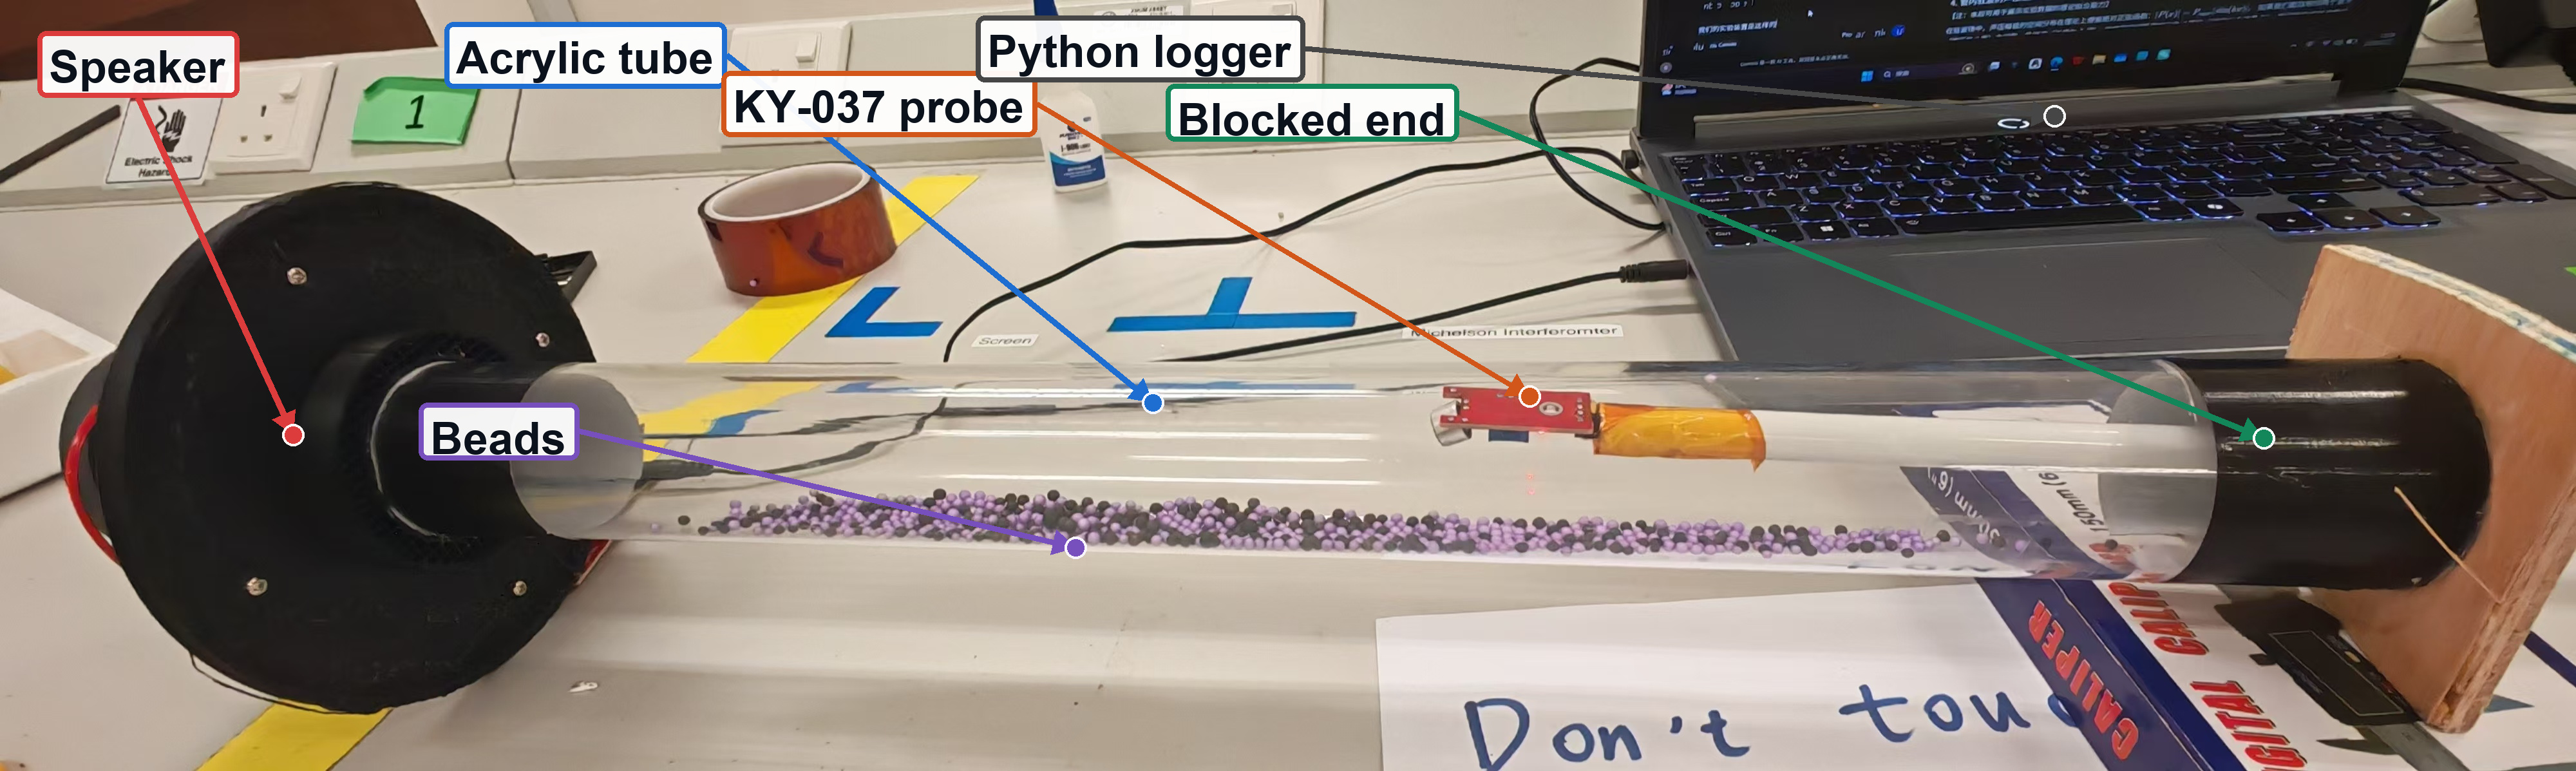
\includegraphics[width=0.96\linewidth]{setup_overview.jpg}
  \caption{Full experimental setup. The loudspeaker on the left drives the acrylic tube. The blocked end board, movable KY-037 microphone probe, beads, and laptop/Python logger form the measurement side of the apparatus.}
  \label{fig:full-setup}
\end{figure}

\begin{figure}[H]
  \centering
  \begin{subfigure}{0.47\linewidth}
    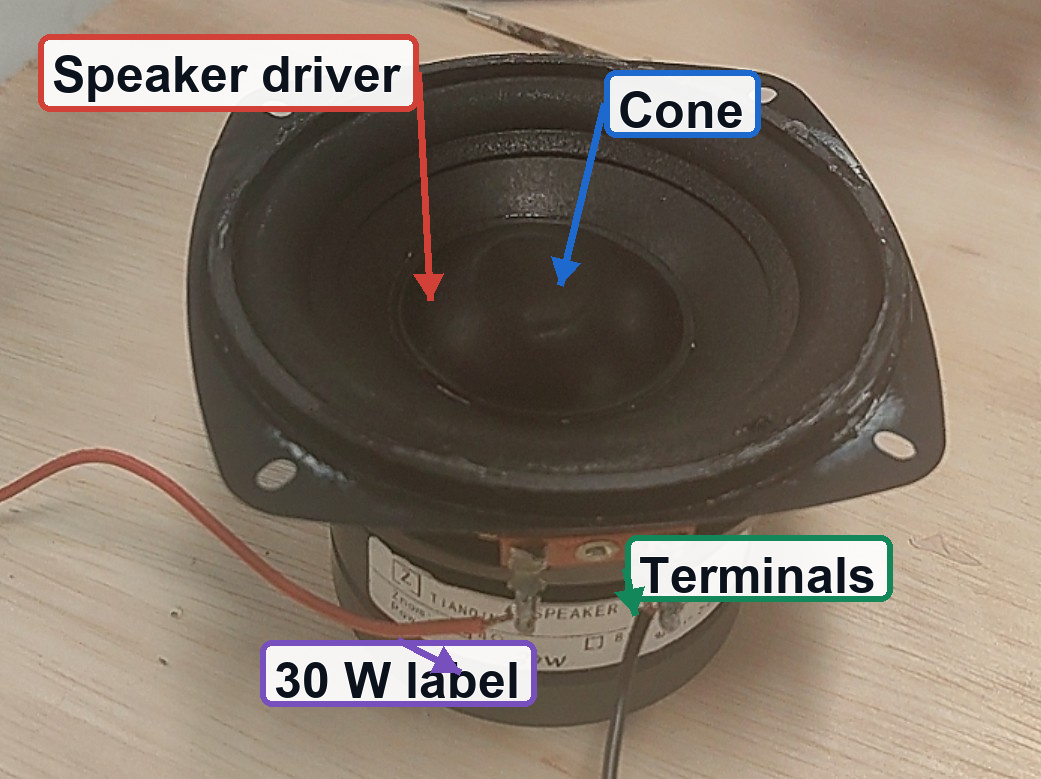
\includegraphics[width=\linewidth]{subwoofer_driver.jpg}
    \caption{Loudspeaker driver used to excite acoustic waves in the tube.}
  \end{subfigure}
  \hfill
  \begin{subfigure}{0.47\linewidth}
    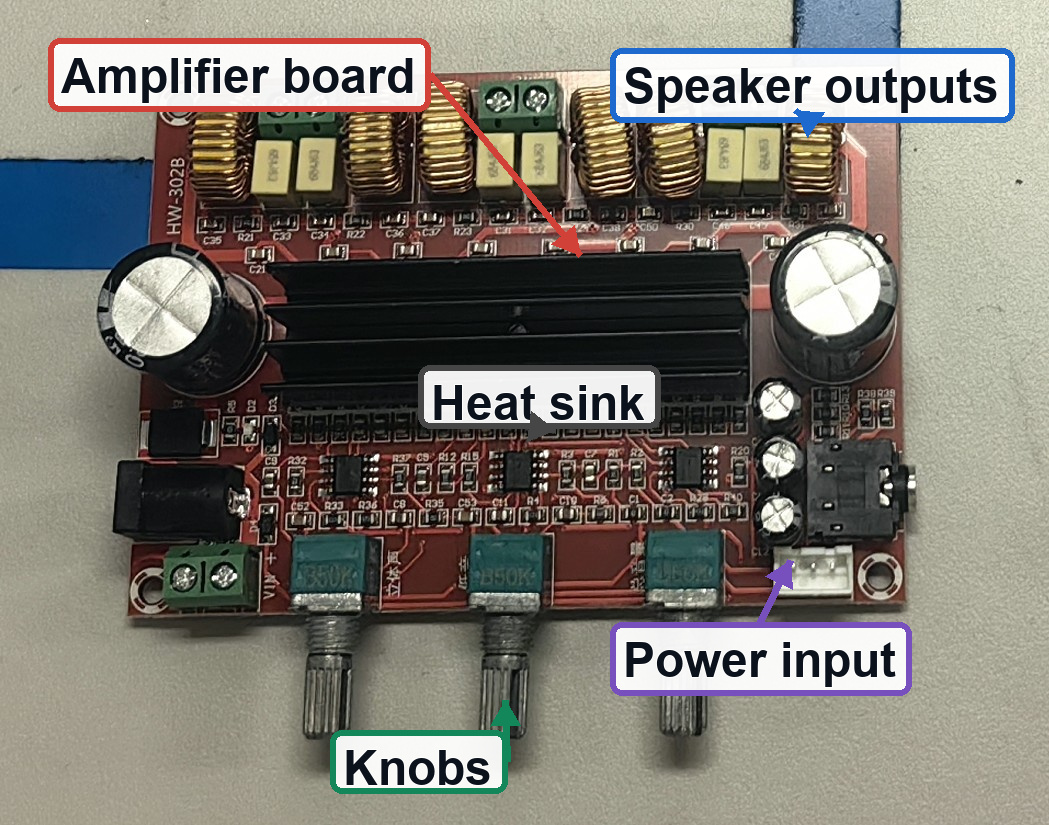
\includegraphics[width=\linewidth]{amplifier_board.jpg}
    \caption{Audio amplifier board used between the tone source and the loudspeaker.}
  \end{subfigure}
  \caption{Drive-chain components. The loudspeaker converts the amplified electrical signal into acoustic excitation. The amplifier board provides the adjustable drive signal for the speaker.}
  \label{fig:drive-components}
\end{figure}

\section{Experimental Method}

\subsection{Bead Visualization}

At selected frequencies, beads inside the transparent tube were photographed. These images were not processed as quantitative bead-tracking data. They were used to check whether the visible bead distribution changed with frequency and whether higher frequencies produced more separated spatial groups.

\subsection{Fixed-Position Frequency Sweep}

For the sweep, the microphone was held near \(x_0=\SI{37.5}{cm}\) while the drive frequency was varied. The expected diagnostic result was that response features might appear near modal frequencies. But the fixed-position amplitude should be read as
\begin{equation}
  \fixedamp(f,x_0)\approx S(f)M(f)R_{\mathrm{tube}}(f)\left|P_f(x_0)\right|,
\end{equation}
where \(S(f)\) is the source and speaker response, \(M(f)\) is the microphone/electronics response, \(R_{\mathrm{tube}}(f)\) is the tube response, and \(\left|P_f(x_0)\right|\) is the local pressure amplitude at the chosen point. For this reason, the sweep is useful but not sufficient as mode-shape evidence.

\subsection{Frequency-Position Mapping}

For each selected frequency, the microphone was moved through accessible positions along the tube. The final cleaned analysis table contains 43 positions per frequency from \SI{1}{cm} to \SI{43}{cm}. The six frequencies were \SI{170}{Hz}, \SI{255}{Hz}, \SI{343}{Hz}, \SI{425}{Hz}, \SI{510}{Hz} and \SI{680}{Hz}. Each position-frequency point summarizes a short capture window using median RMS amplitude. The standard deviation and clipping counts were kept for quality checking. Three missing \SI{255}{Hz} positions, \SI{35}{cm}, \SI{36}{cm} and \SI{42}{cm}, were filled by linear interpolation in the final presentation analysis and were explicitly marked in the plot outputs.

\section{Results}

\subsection{Qualitative Bead Visualization}

The bead photographs showed frequency-dependent spatial patterns. At lower frequencies, the visible bead distribution was broader and less segmented. At higher frequencies, especially around \SI{510}{Hz} and \SI{680}{Hz}, more separated bead groups were visible. This supports the presence of frequency-dependent acoustic behavior. But it is not treated as quantitative pressure data because bead motion can emphasize particle-motion patterns rather than the pressure envelope measured by the microphone.

\begin{figure}[H]
  \centering
  \begin{subfigure}{0.32\linewidth}
    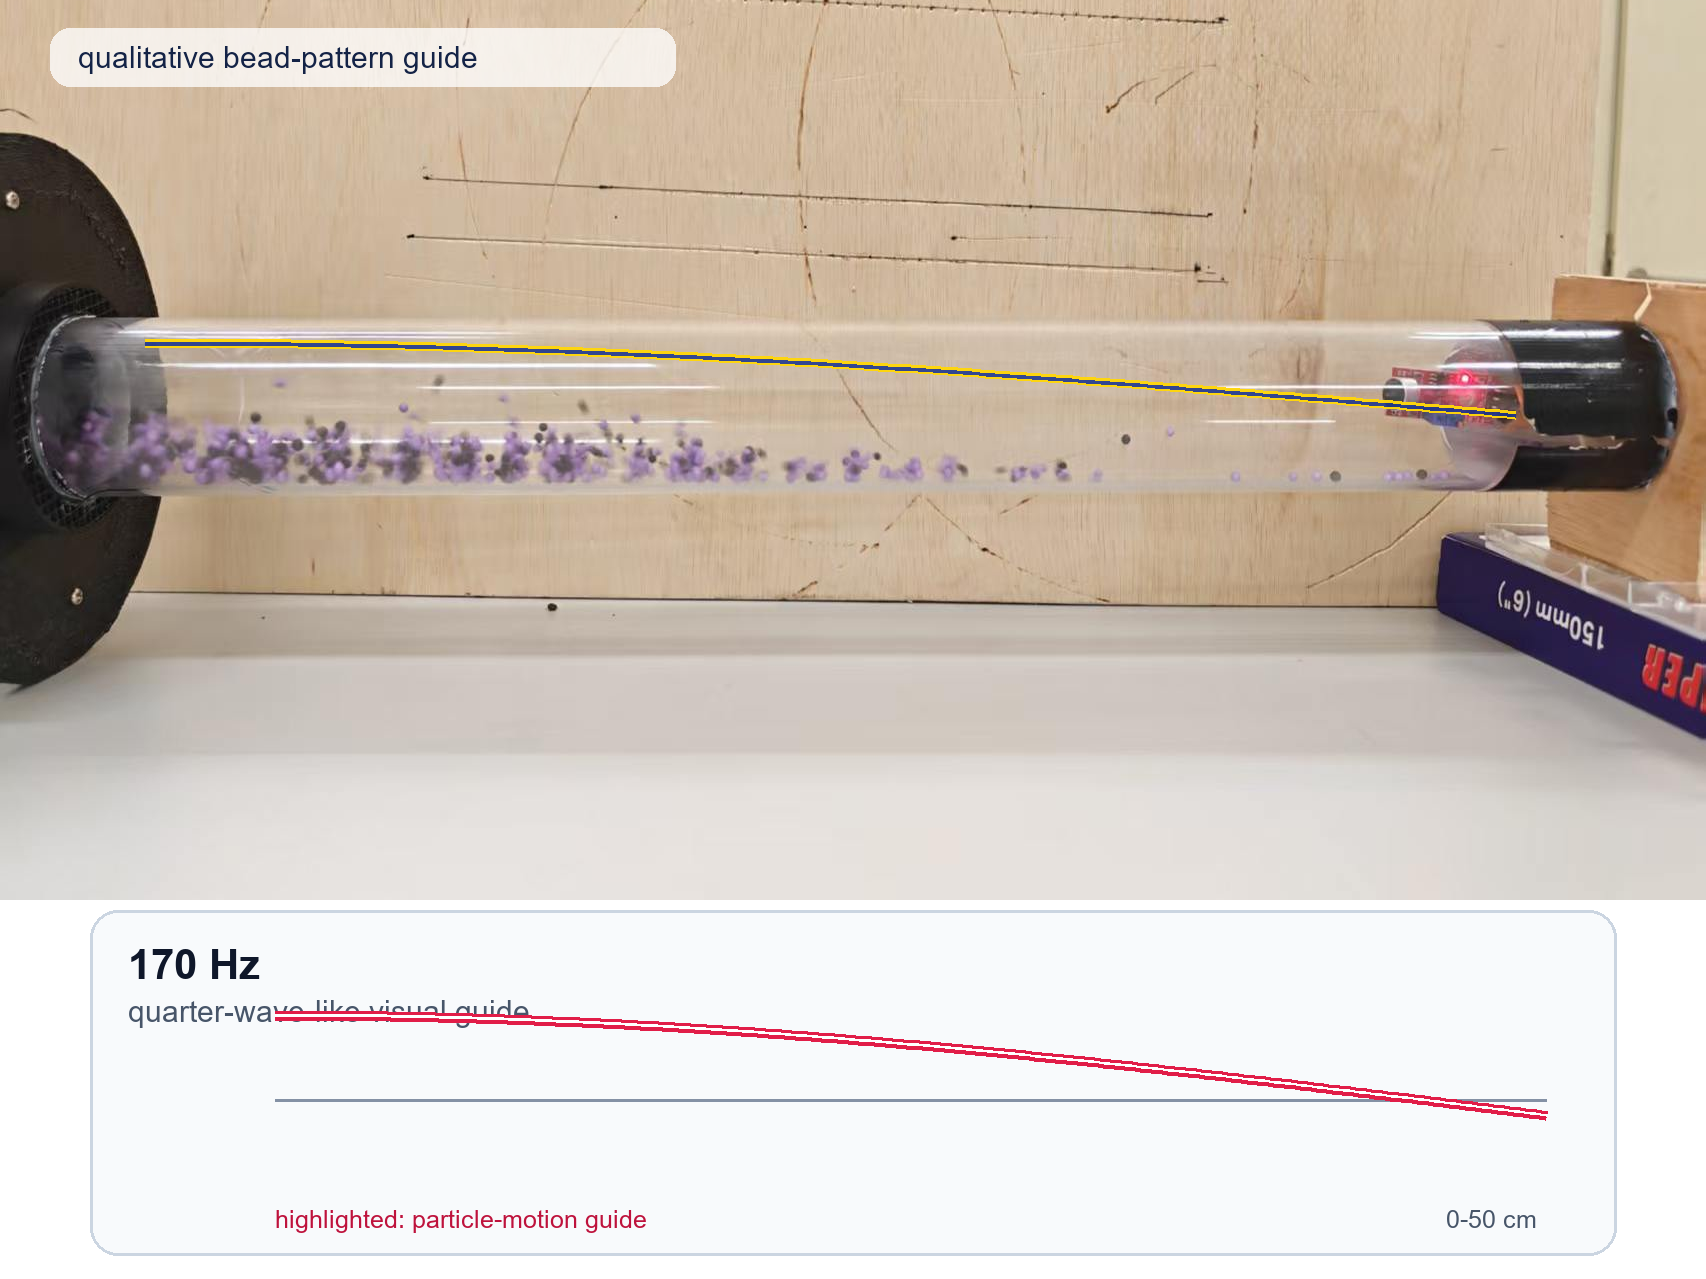
\includegraphics[width=\linewidth]{f170_beads_wave.png}
    \caption{\SI{170}{Hz}}
  \end{subfigure}
  \hfill
  \begin{subfigure}{0.32\linewidth}
    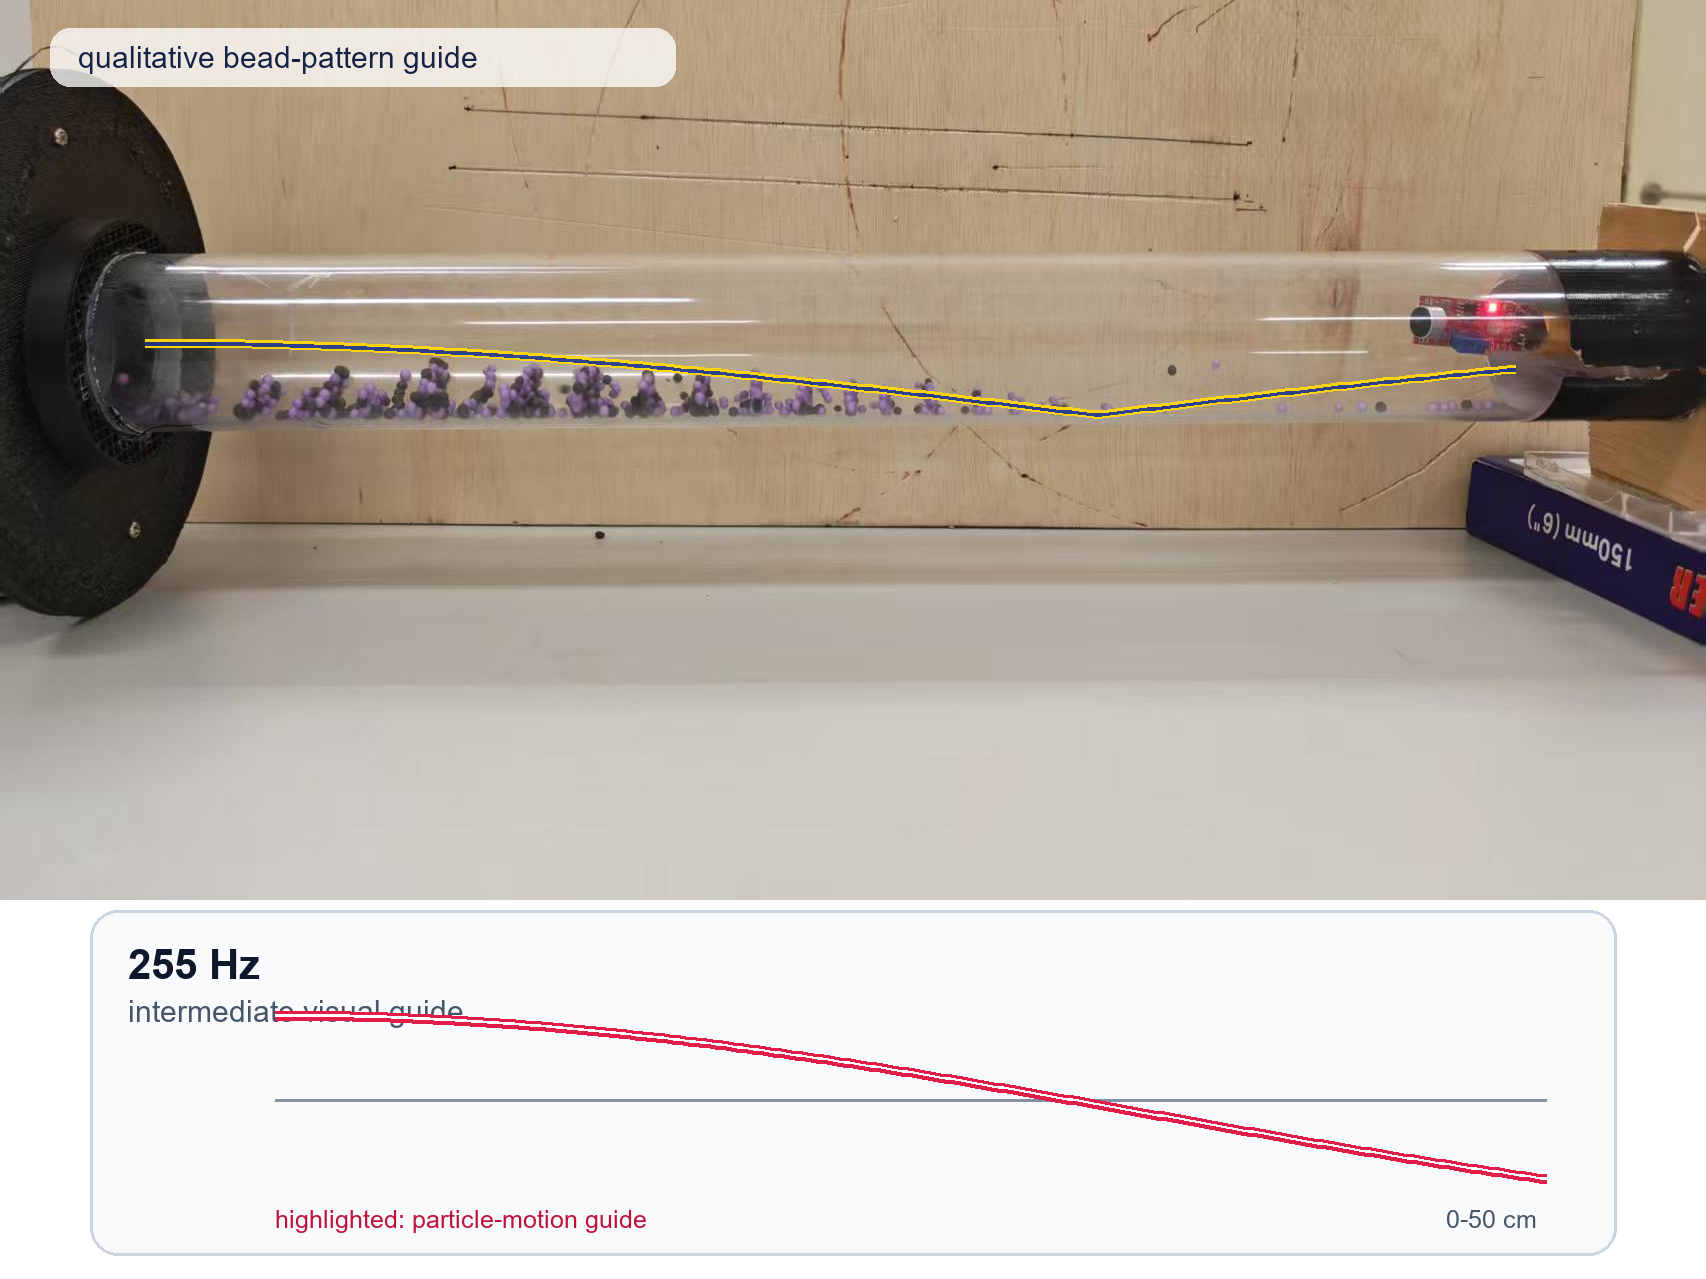
\includegraphics[width=\linewidth]{f255_beads_wave.png}
    \caption{\SI{255}{Hz}}
  \end{subfigure}
  \hfill
  \begin{subfigure}{0.32\linewidth}
    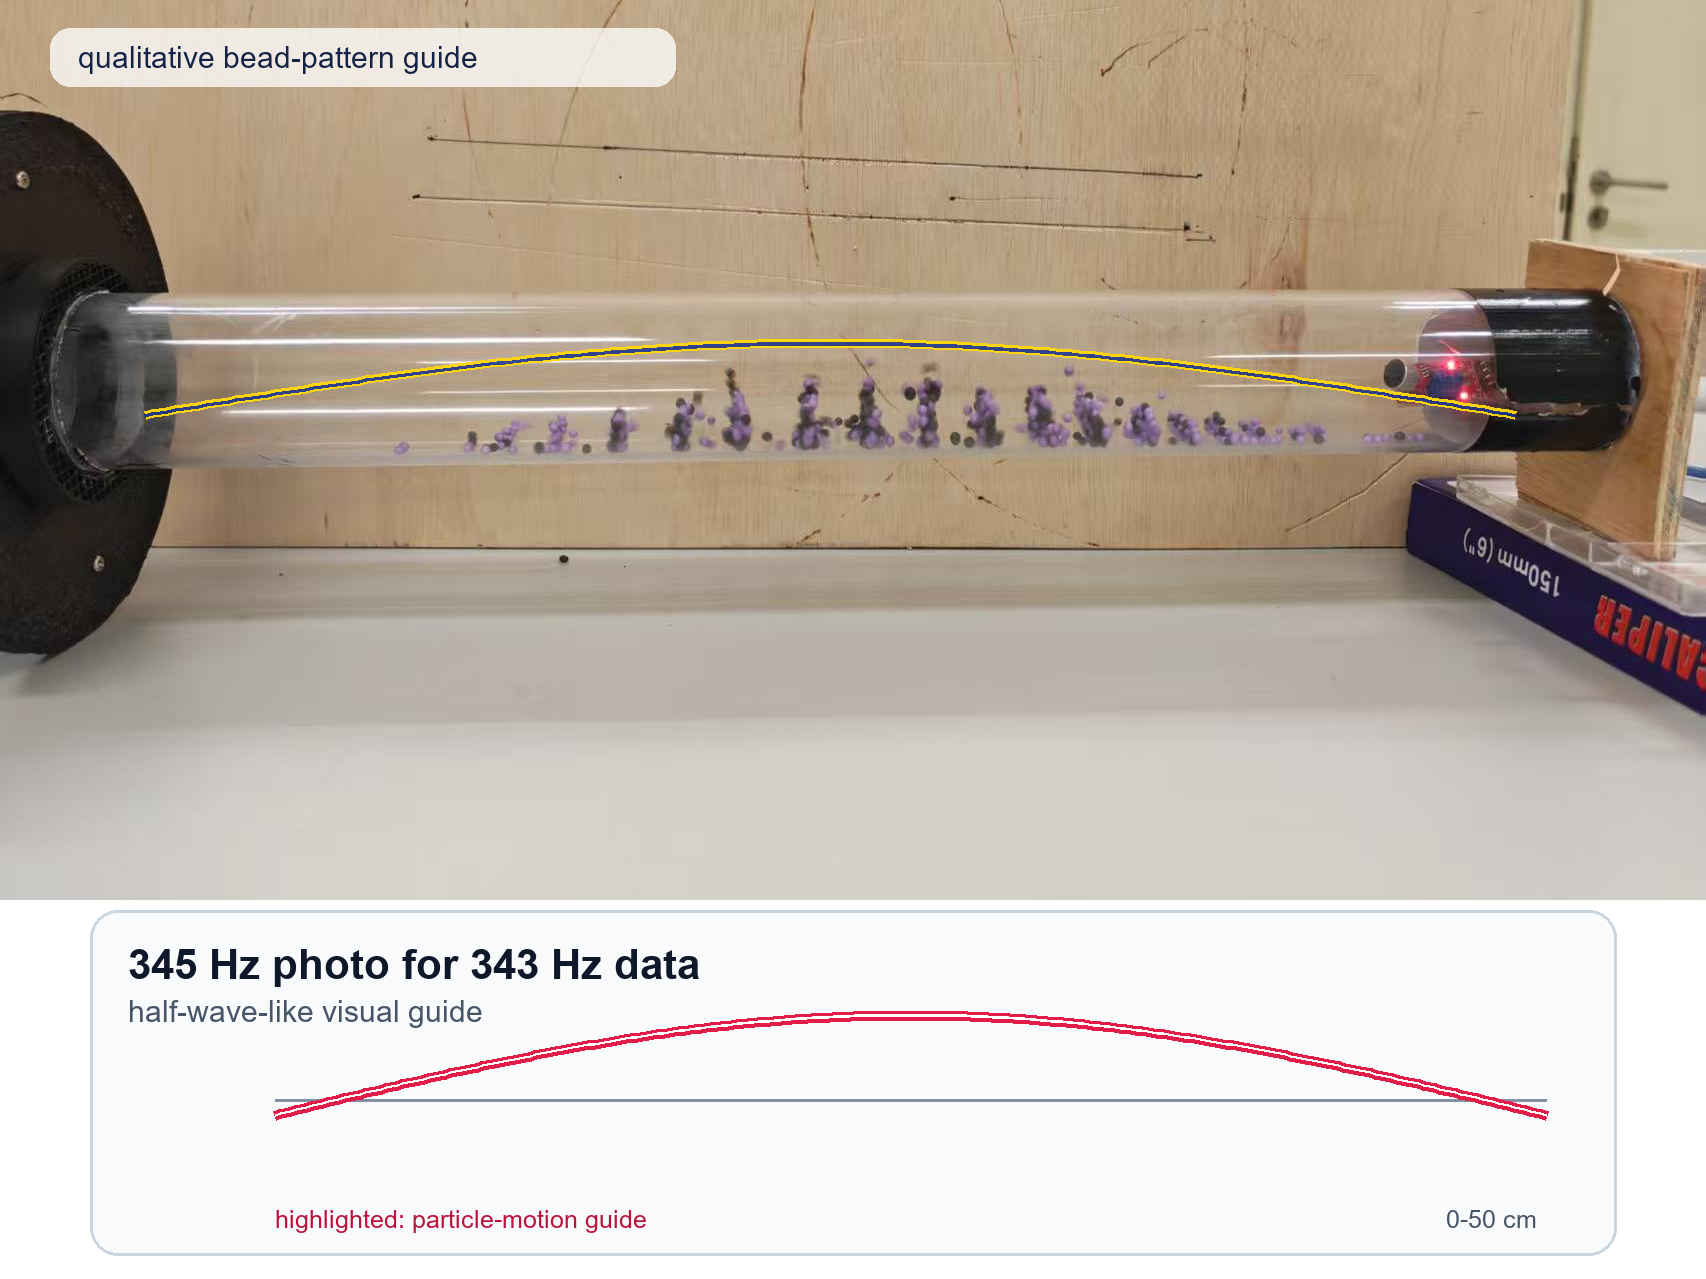
\includegraphics[width=\linewidth]{f345_beads_wave.png}
    \caption{\SI{345}{Hz} visual reference for \SI{343}{Hz} data}
  \end{subfigure}

  \vspace{0.4em}

  \begin{subfigure}{0.32\linewidth}
    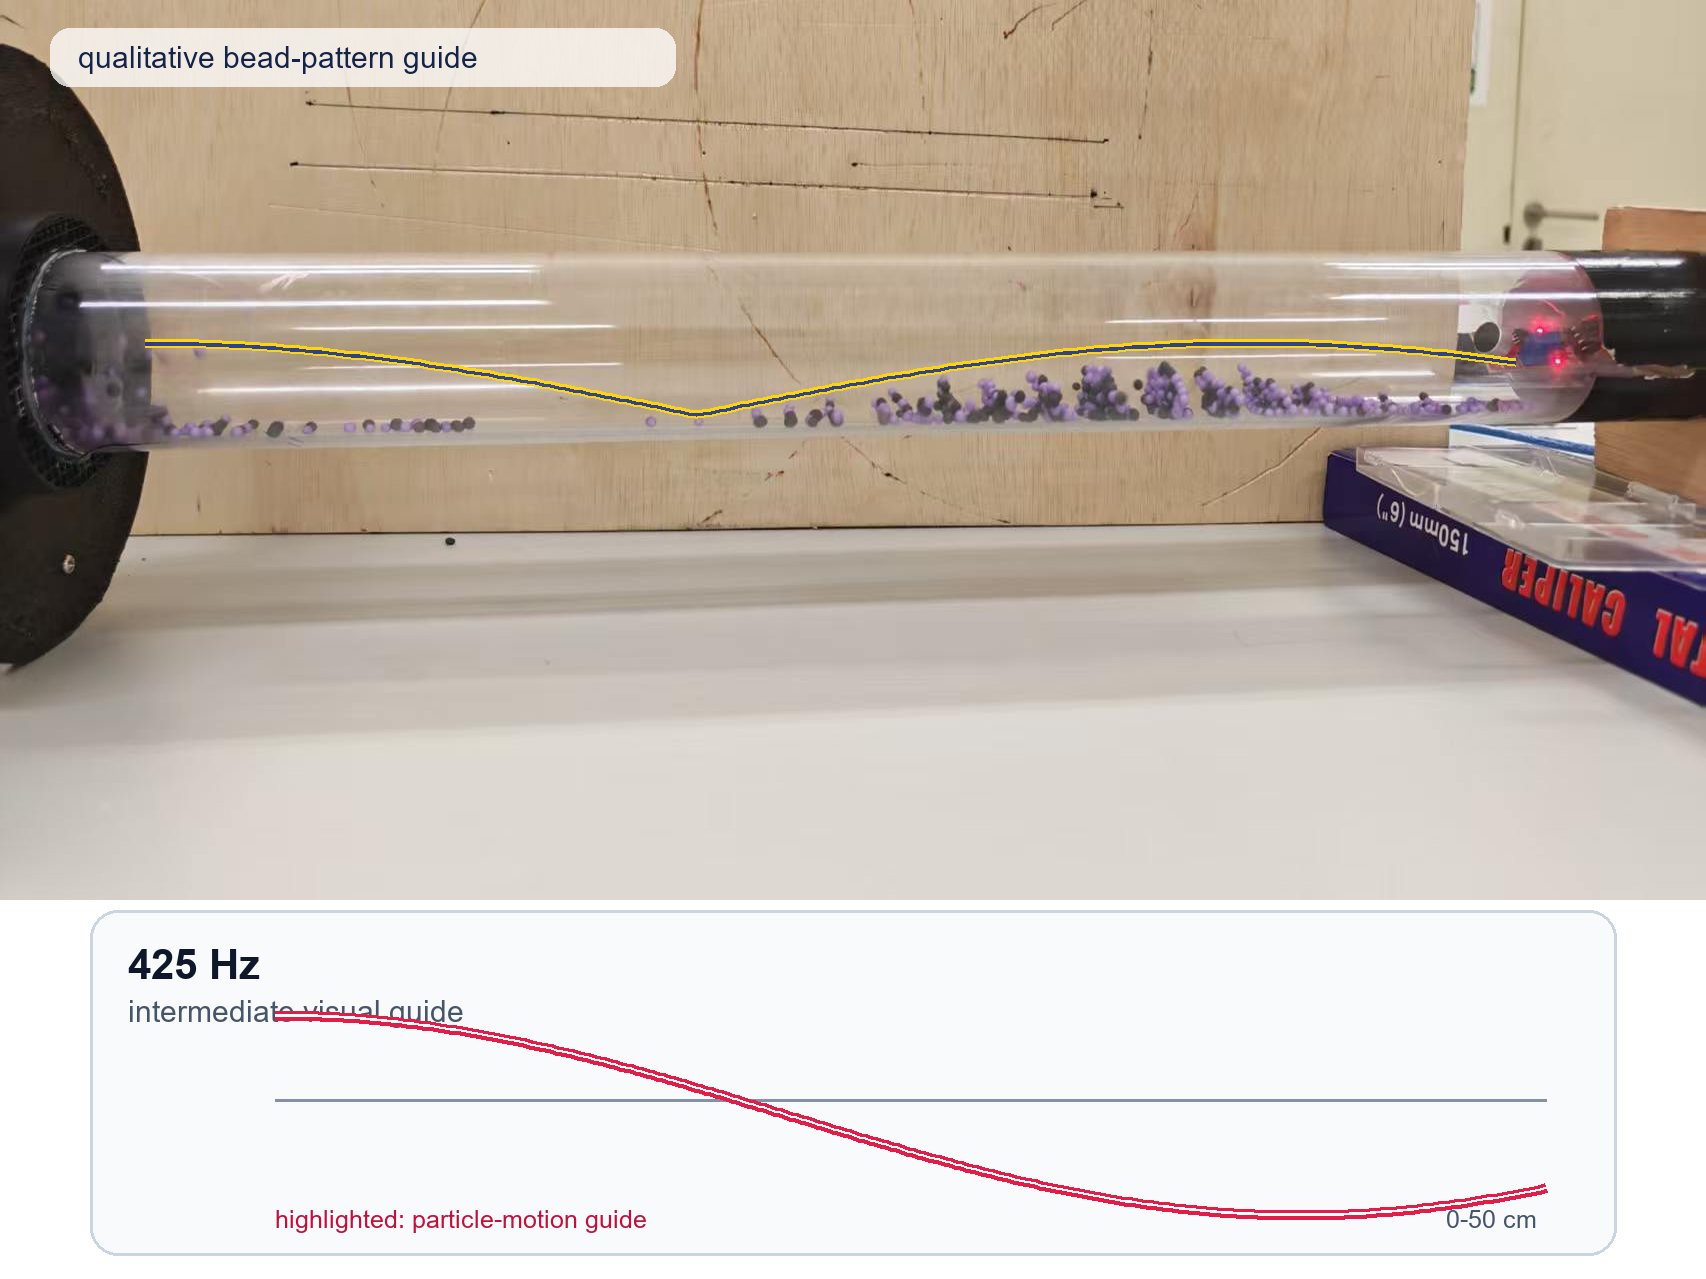
\includegraphics[width=\linewidth]{f425_beads_wave.png}
    \caption{\SI{425}{Hz}}
  \end{subfigure}
  \hfill
  \begin{subfigure}{0.32\linewidth}
    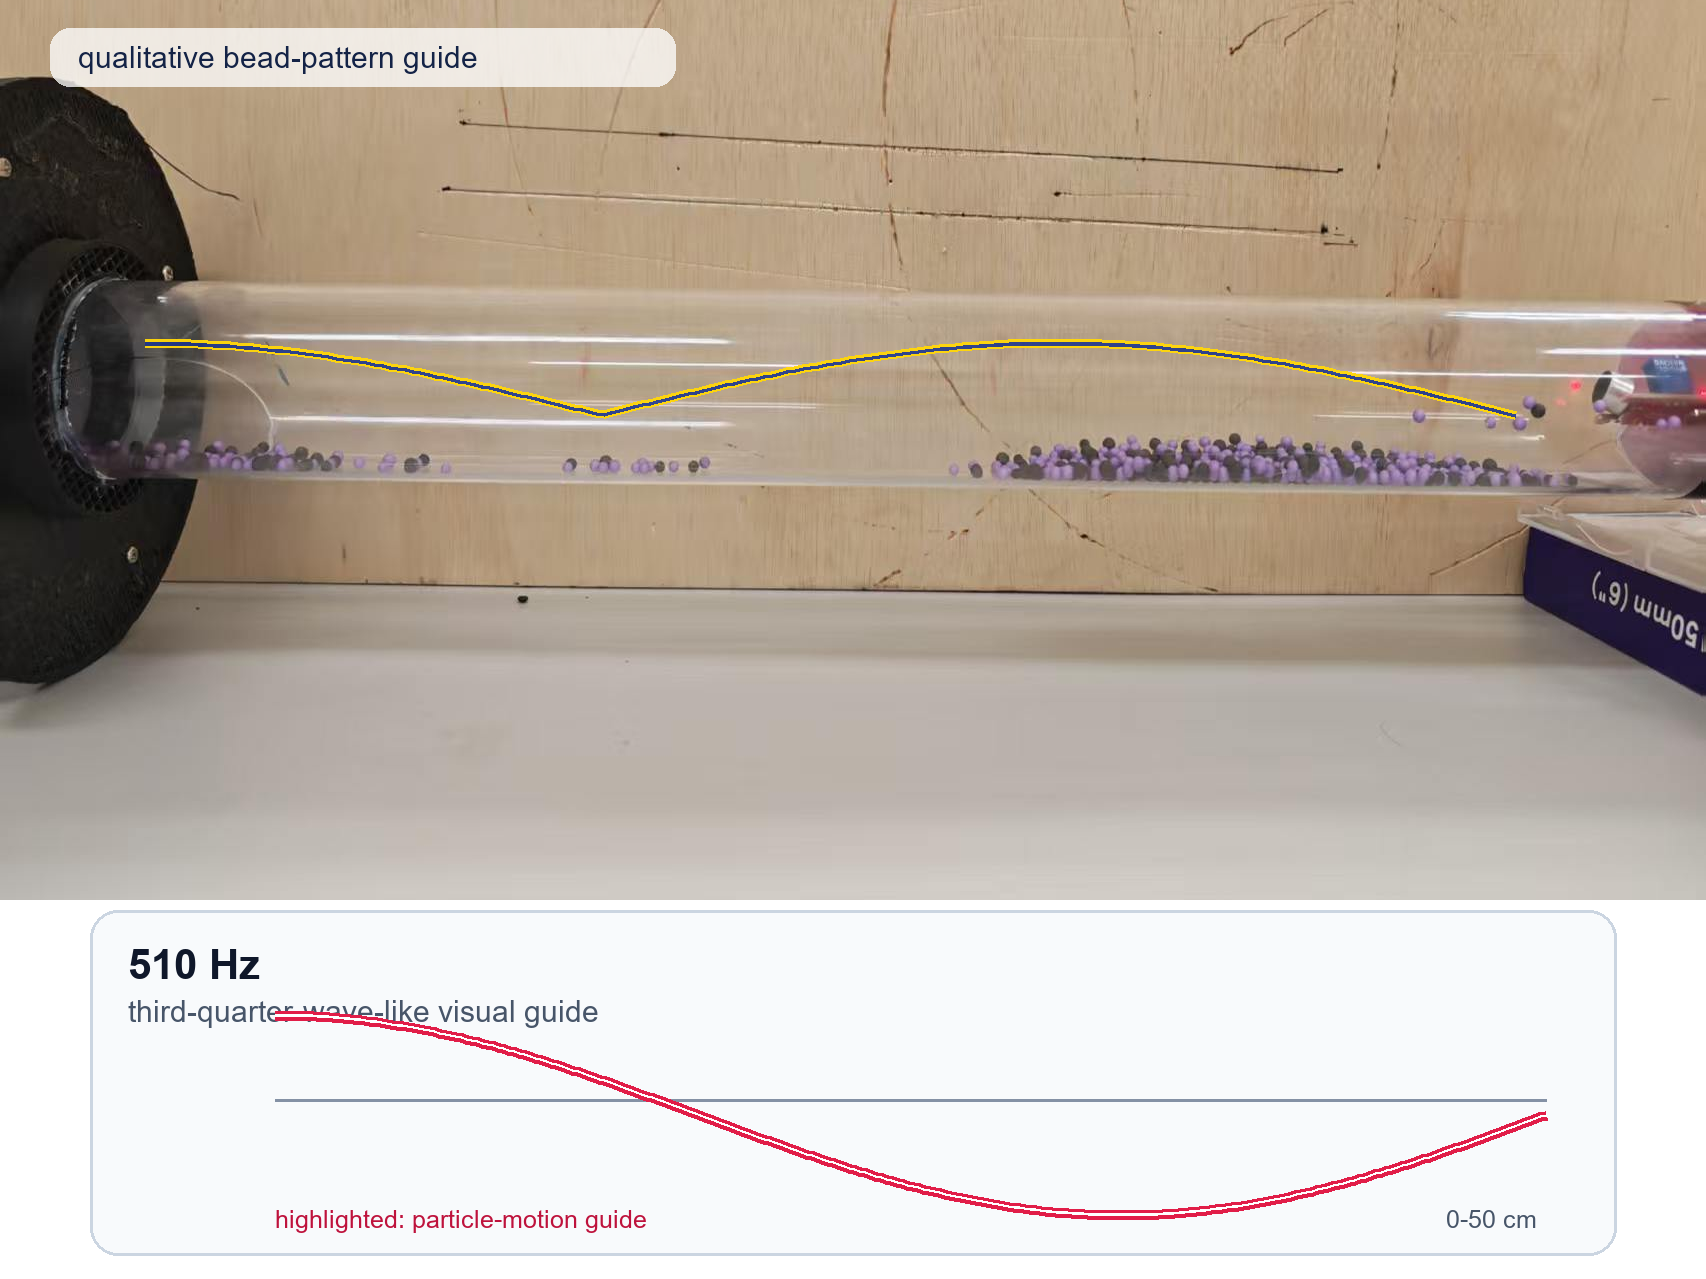
\includegraphics[width=\linewidth]{f510_beads_wave.png}
    \caption{\SI{510}{Hz}}
  \end{subfigure}
  \hfill
  \begin{subfigure}{0.32\linewidth}
    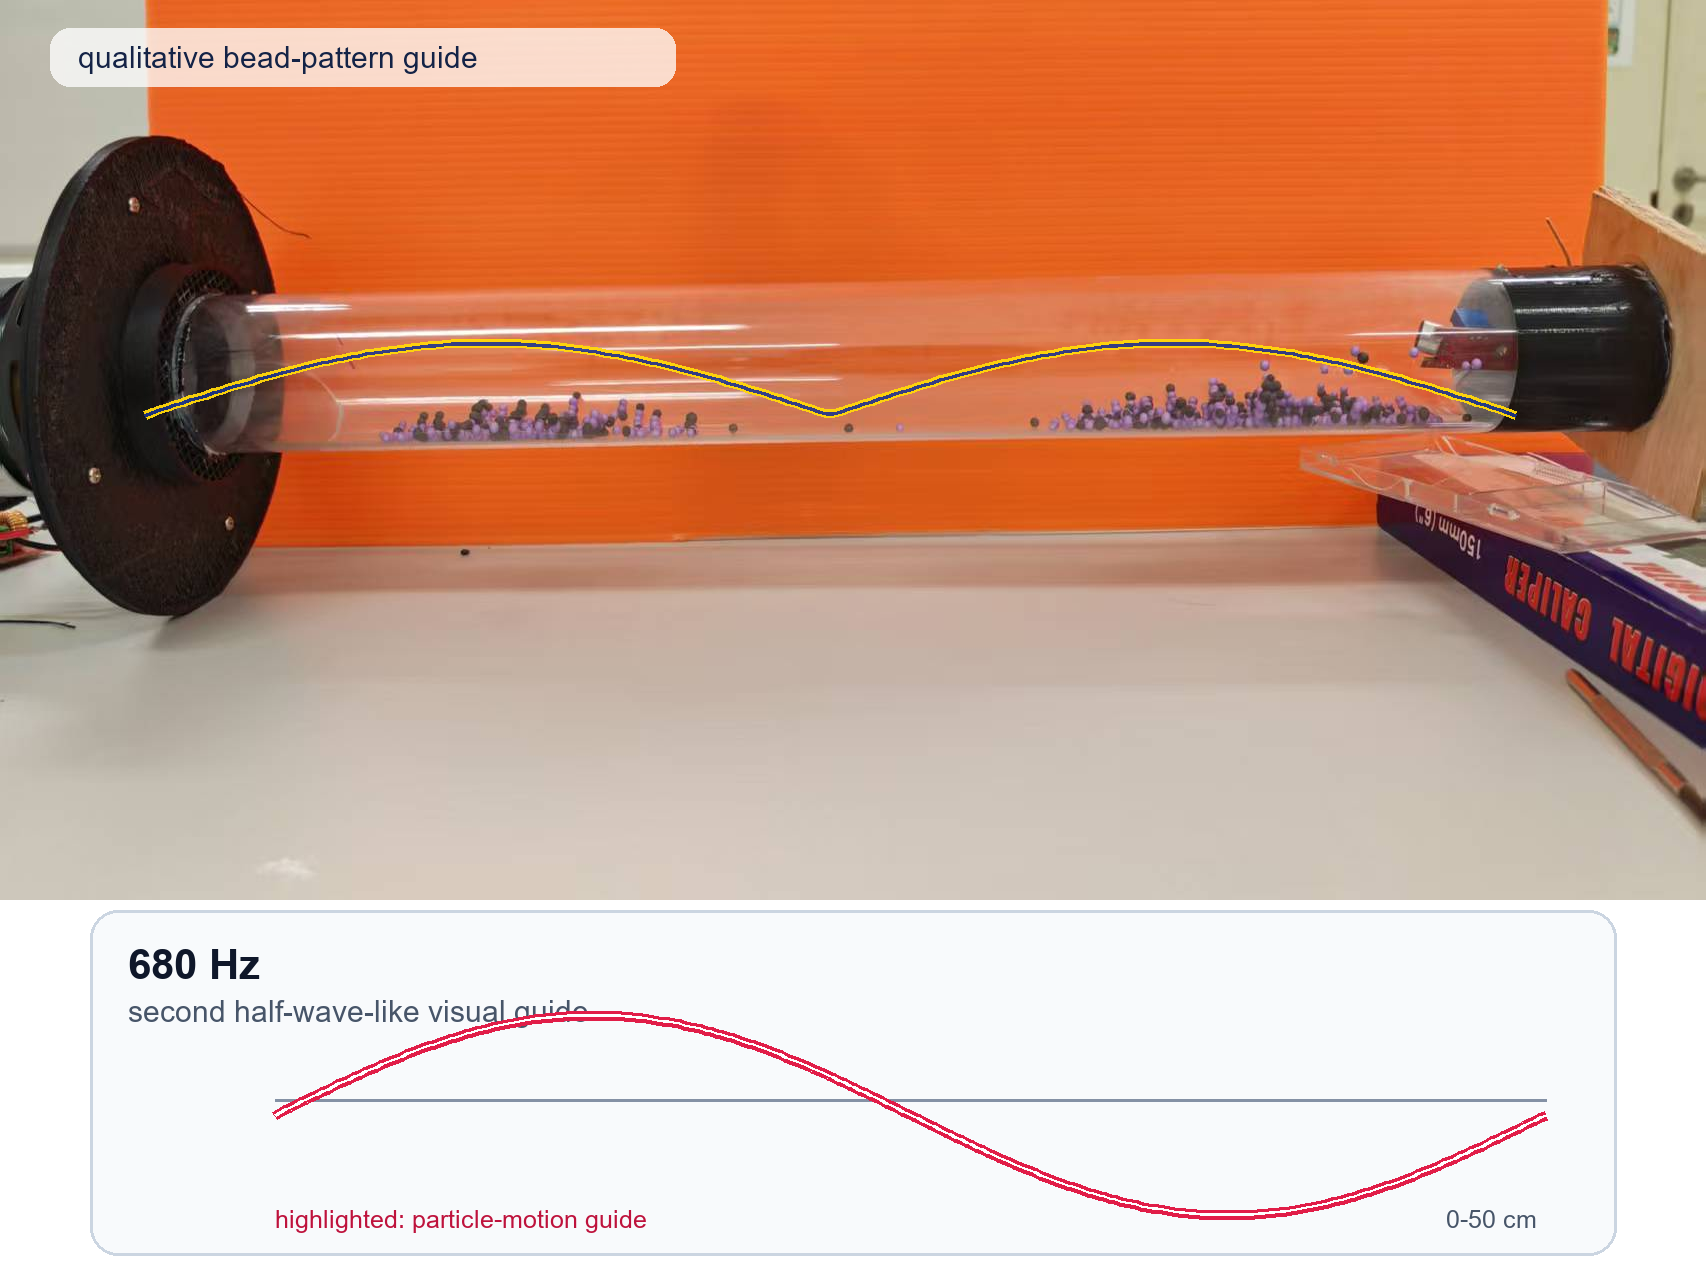
\includegraphics[width=\linewidth]{f680_beads_wave.png}
    \caption{\SI{680}{Hz}}
  \end{subfigure}
  \caption{Bead visualization images with particle-motion guide overlays. These images are qualitative visual support, not quantitative bead tracking.}
\end{figure}

\subsection{Fixed-Position Frequency Sweep}

The fixed-position sweep did not produce a clean textbook resonance spectrum. The strongest median amplitudes occurred in the broad low-frequency region. The largest values were around \SIrange{120}{160}{Hz}, with a maximum at \SI{140}{Hz}. Additional local maxima appeared around \SI{250}{Hz} and \SI{390}{Hz}. The selected principal frequencies at \SI{343}{Hz} and \SI{510}{Hz} had much lower fixed-position amplitudes than \SI{170}{Hz} at the chosen \(x=\SI{37.5}{cm}\). This is consistent with the idea that a single probe position can be close to a local low-amplitude region for a particular mode shape.

\begin{figure}[H]
  \centering
  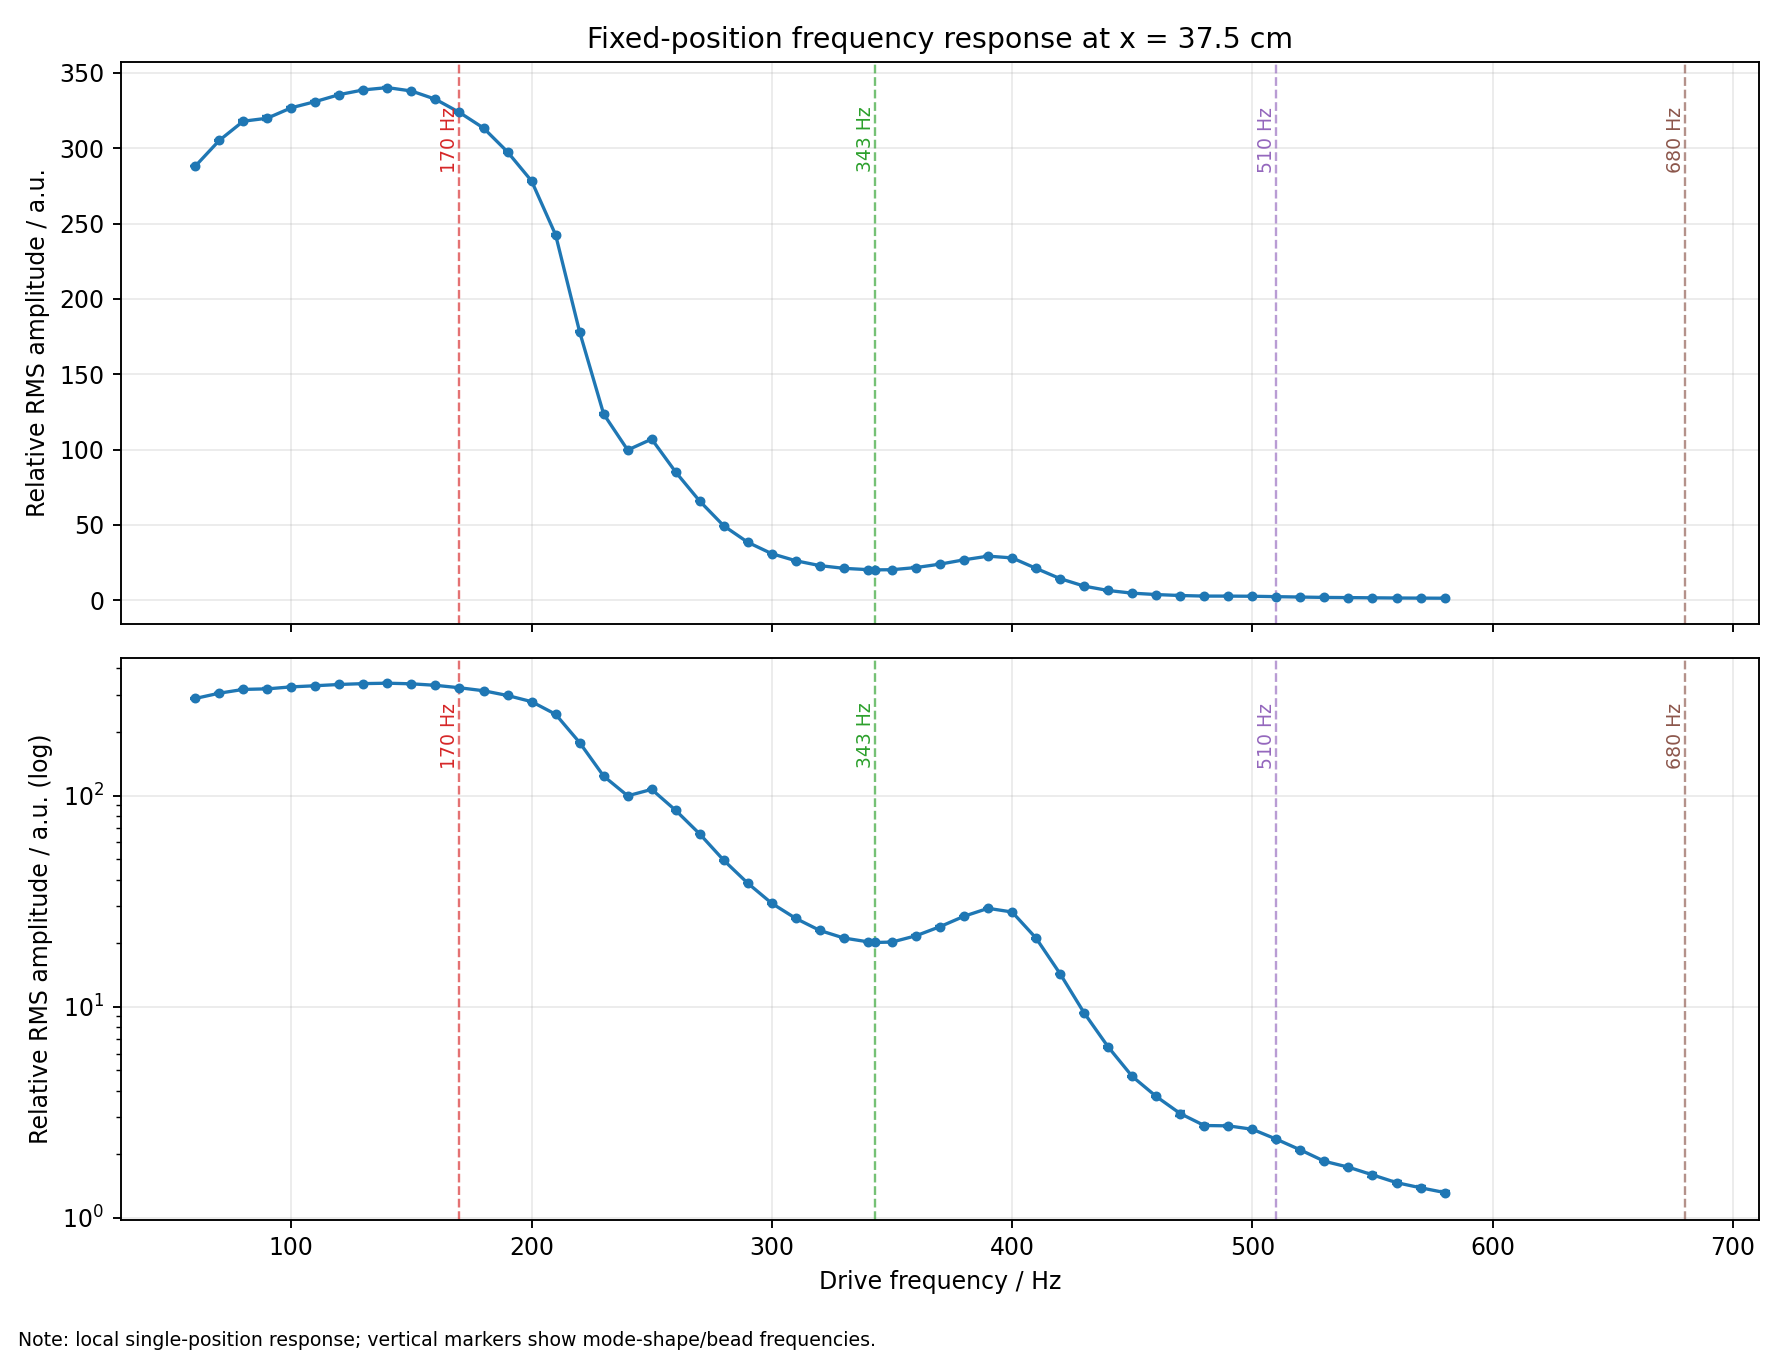
\includegraphics[width=0.92\linewidth]{frequency_response_x37p5.png}
  \caption{Fixed-position frequency response at \(x=\SI{37.5}{cm}\). This plot is a diagnostic response curve, not a full mode-shape measurement.}
\end{figure}

\begin{table}[H]
  \centering
  \caption{Fixed-position sweep values for selected frequencies that appear in the sweep table.}
  \begin{tabular}{lrrr}
    \toprule
    Frequency & Median amplitude & Standard deviation & Clipped samples \\
    \midrule
    \SI{170}{Hz} & 323.71 & 0.294 & 0 \\
    \SI{343}{Hz} & 20.15 & 0.077 & 0 \\
    \SI{510}{Hz} & 2.36 & 0.024 & 0 \\
    \SI{425}{Hz}, \SI{680}{Hz} & \multicolumn{3}{l}{not directly sampled in this sweep table} \\
    \bottomrule
  \end{tabular}
\end{table}

\begin{table}[H]
  \centering
  \caption{Eight largest median amplitudes in the \(x=\SI{37.5}{cm}\) sweep; the broad low-frequency response dominates.}
  \begin{tabular}{rrr}
    \toprule
    Top sweep frequency & Median amplitude & Standard deviation \\
    \midrule
    140 & 340.21 & 0.248 \\
    130 & 338.69 & 0.189 \\
    150 & 337.96 & 0.121 \\
    120 & 335.57 & 0.172 \\
    160 & 332.48 & 0.166 \\
    110 & 330.93 & 0.284 \\
    100 & 326.82 & 0.355 \\
    170 & 323.71 & 0.294 \\
    \bottomrule
  \end{tabular}
\end{table}

\subsection{Frequency-Position RMS Mapping}

The frequency-position map is the main quantitative result. Each frequency row was normalized by its own maximum. After this normalization, the heatmap and line plots showed that high- and low-amplitude regions shift with drive frequency. The accessible scan length in the cleaned analysis is \SIrange{1}{43}{cm}, not the full \SI{50}{cm} tube length. Therefore, the measured mode shapes should be interpreted over the actual scanned region.

\begin{figure}[H]
  \centering
  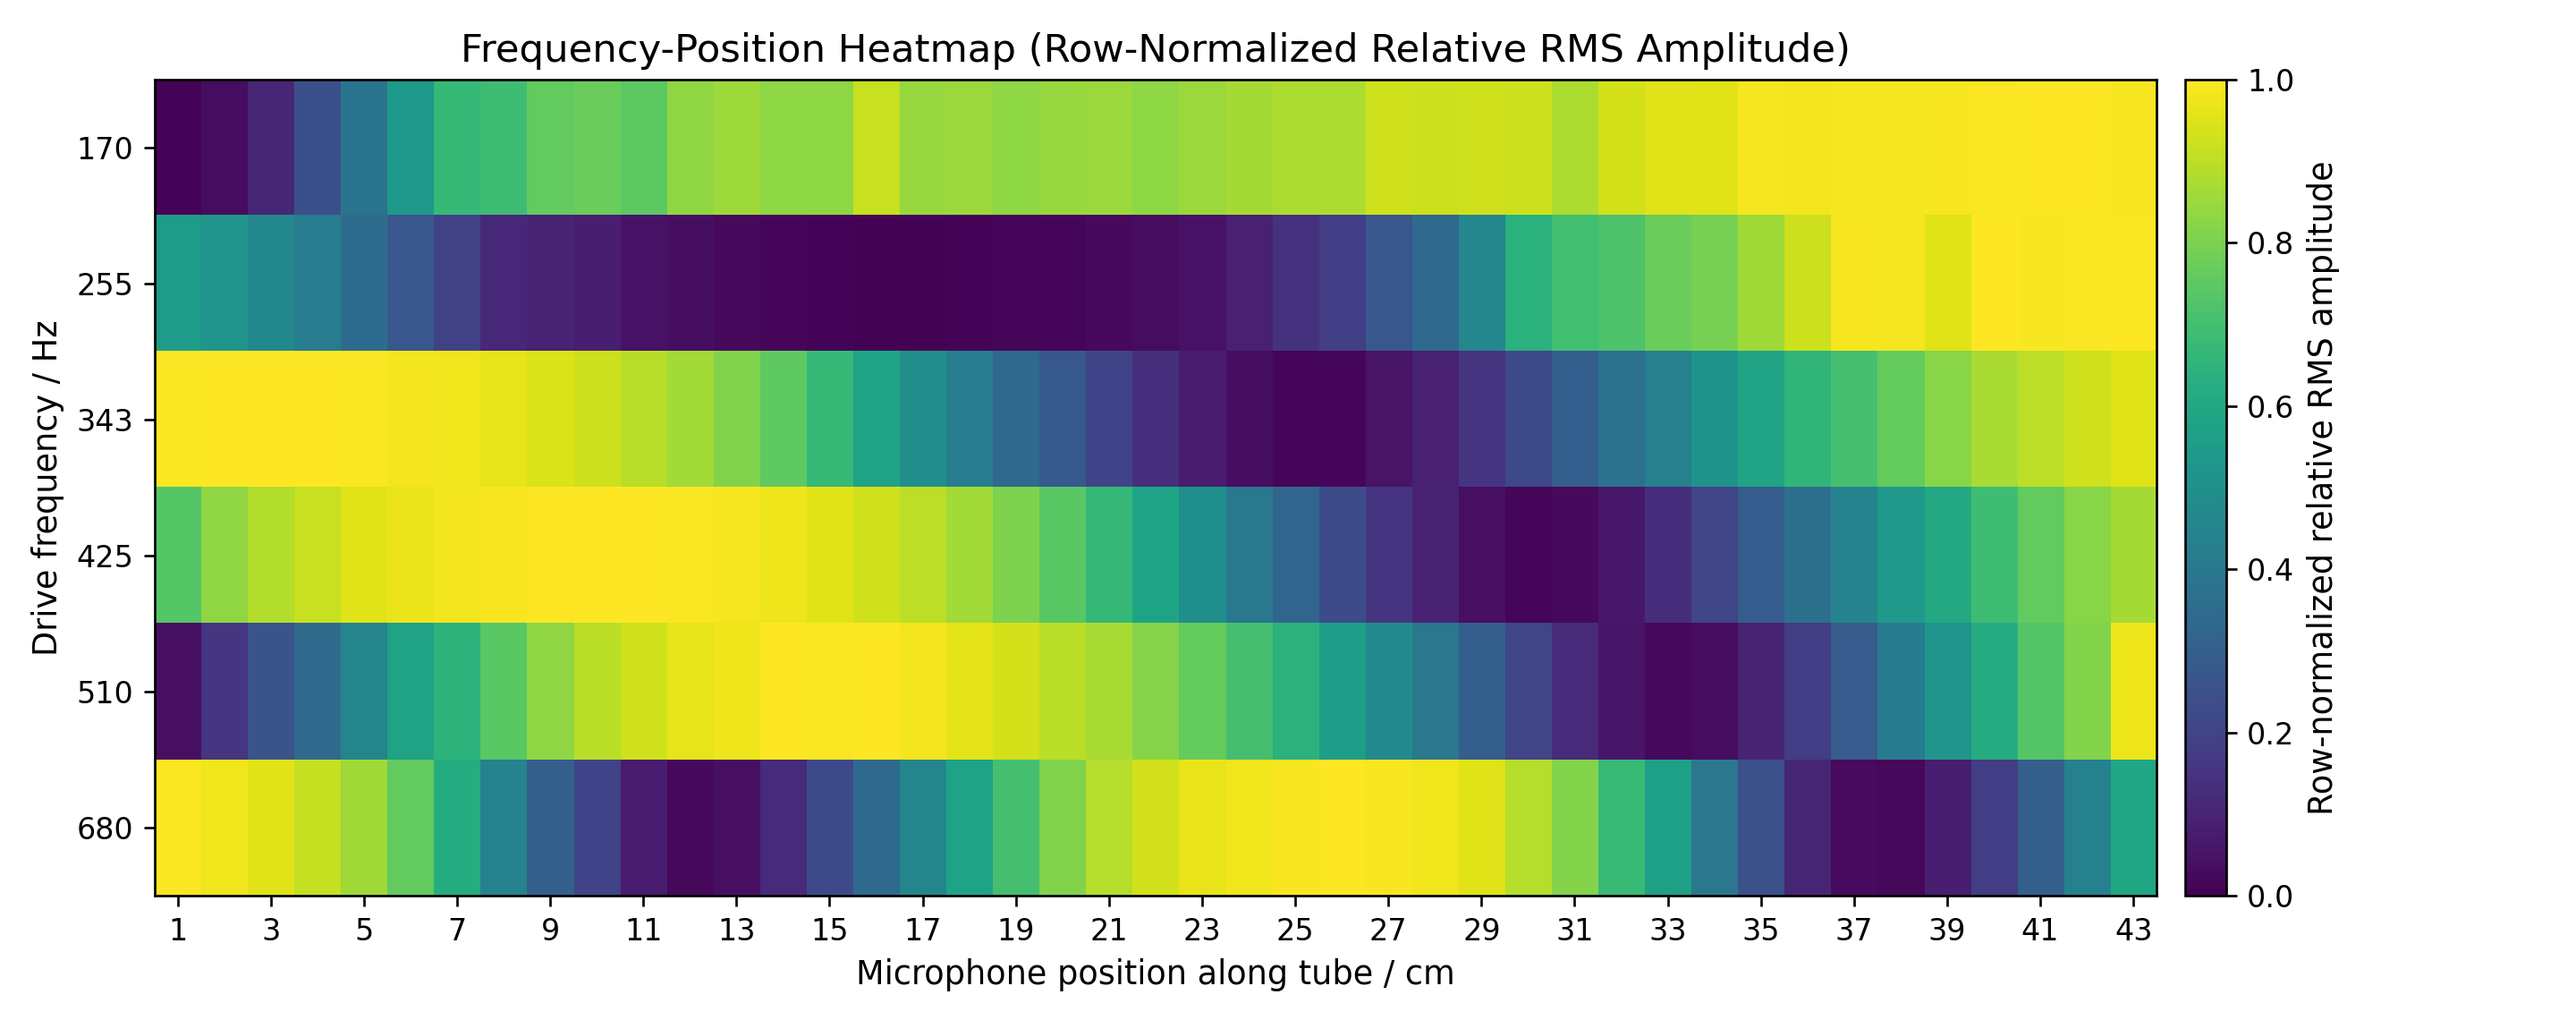
\includegraphics[width=0.92\linewidth]{mode_shape_6freq_filled_row_normalized_heatmap.png}
  \caption{Row-normalized frequency-position heatmap for \SI{170}{Hz}, \SI{255}{Hz}, \SI{343}{Hz}, \SI{425}{Hz}, \SI{510}{Hz} and \SI{680}{Hz}.}
\end{figure}

\begin{figure}[H]
  \centering
  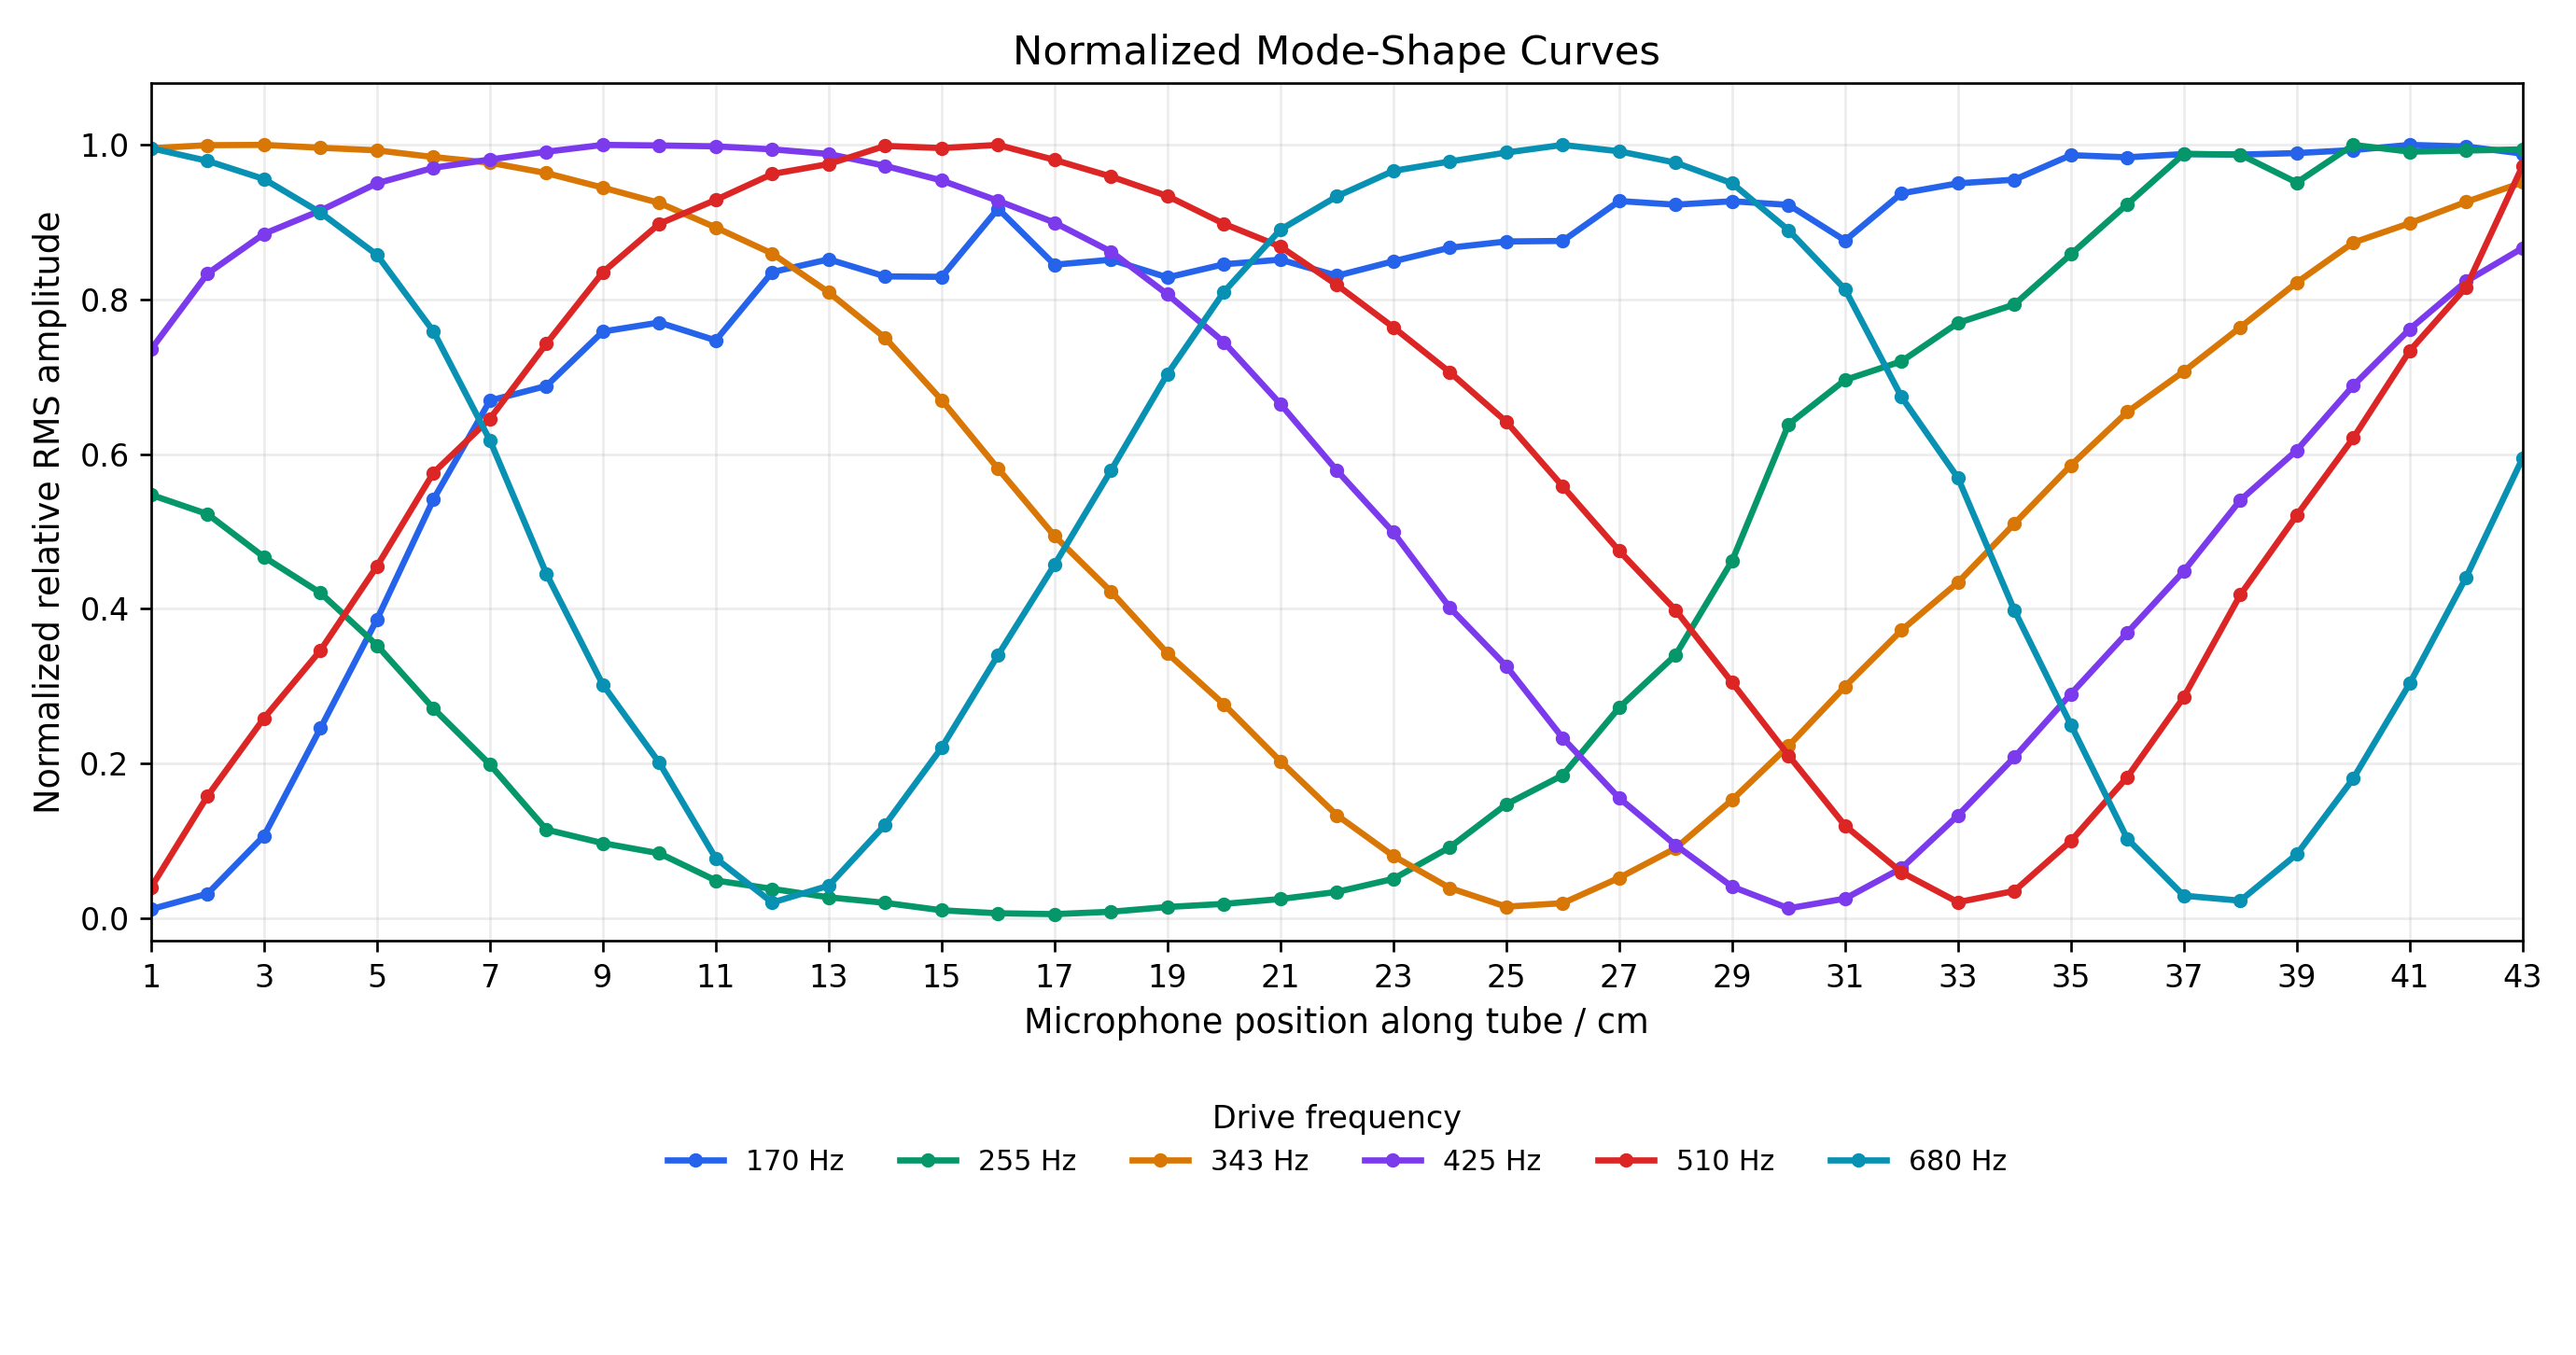
\includegraphics[width=0.92\linewidth]{mode_shape_6freq_lines.png}
  \caption{Six-frequency normalized mode-shape overview. The curves compare spatial pressure-amplitude envelopes after per-frequency normalization.}
\end{figure}

\begin{table}[H]
  \centering
  \caption{Summary of the cleaned six-frequency position-mapping data. Raw median amplitude is in arbitrary sensor units.}
  \scriptsize
  \begin{tabularx}{\linewidth}{>{\raggedleft\arraybackslash}p{1.55cm}
      >{\raggedleft\arraybackslash}p{1.35cm}
      >{\raggedright\arraybackslash}X
      >{\raggedright\arraybackslash}p{2.55cm}
      >{\raggedleft\arraybackslash}p{1.35cm}
      >{\raggedleft\arraybackslash}p{1.55cm}
      >{\raggedleft\arraybackslash}p{1.55cm}}
    \toprule
    Frequency & Positions & Estimated positions & Raw median range & Peak \(x\) & Minimum \(x\) & Minimum \(\anorm\) \\
    \midrule
    170 & 43 & none & 4.07-362.00 & 41 & 1 & 0.011 \\
    255 & 43 & 35, 36, 42 & 1.34-274.39 & 40 & 17 & 0.005 \\
    343 & 43 & none & 5.12-352.35 & 3 & 25 & 0.015 \\
    425 & 43 & none & 4.26-345.08 & 9 & 30 & 0.012 \\
    510 & 43 & none & 6.21-306.27 & 16 & 33 & 0.020 \\
    680 & 43 & none & 6.97-351.25 & 26 & 12 & 0.020 \\
    \bottomrule
  \end{tabularx}
\end{table}

\subsection{Single-Frequency Mode Shapes}

The single-frequency plots compare the measured normalized RMS envelope with an ideal guide. The ideal reference in the final analysis used \(\left|\cos(2\pi f x/v+\phi)\right|\) with \(v=\SI{343}{m.s^{-1}}\), plus fitted phase and linear contrast parameters. This guide is used only for shape comparison because the real speaker-tube boundary is not a perfect textbook open or closed boundary.

\begin{figure}[H]
  \centering
  \begin{subfigure}{0.49\linewidth}
    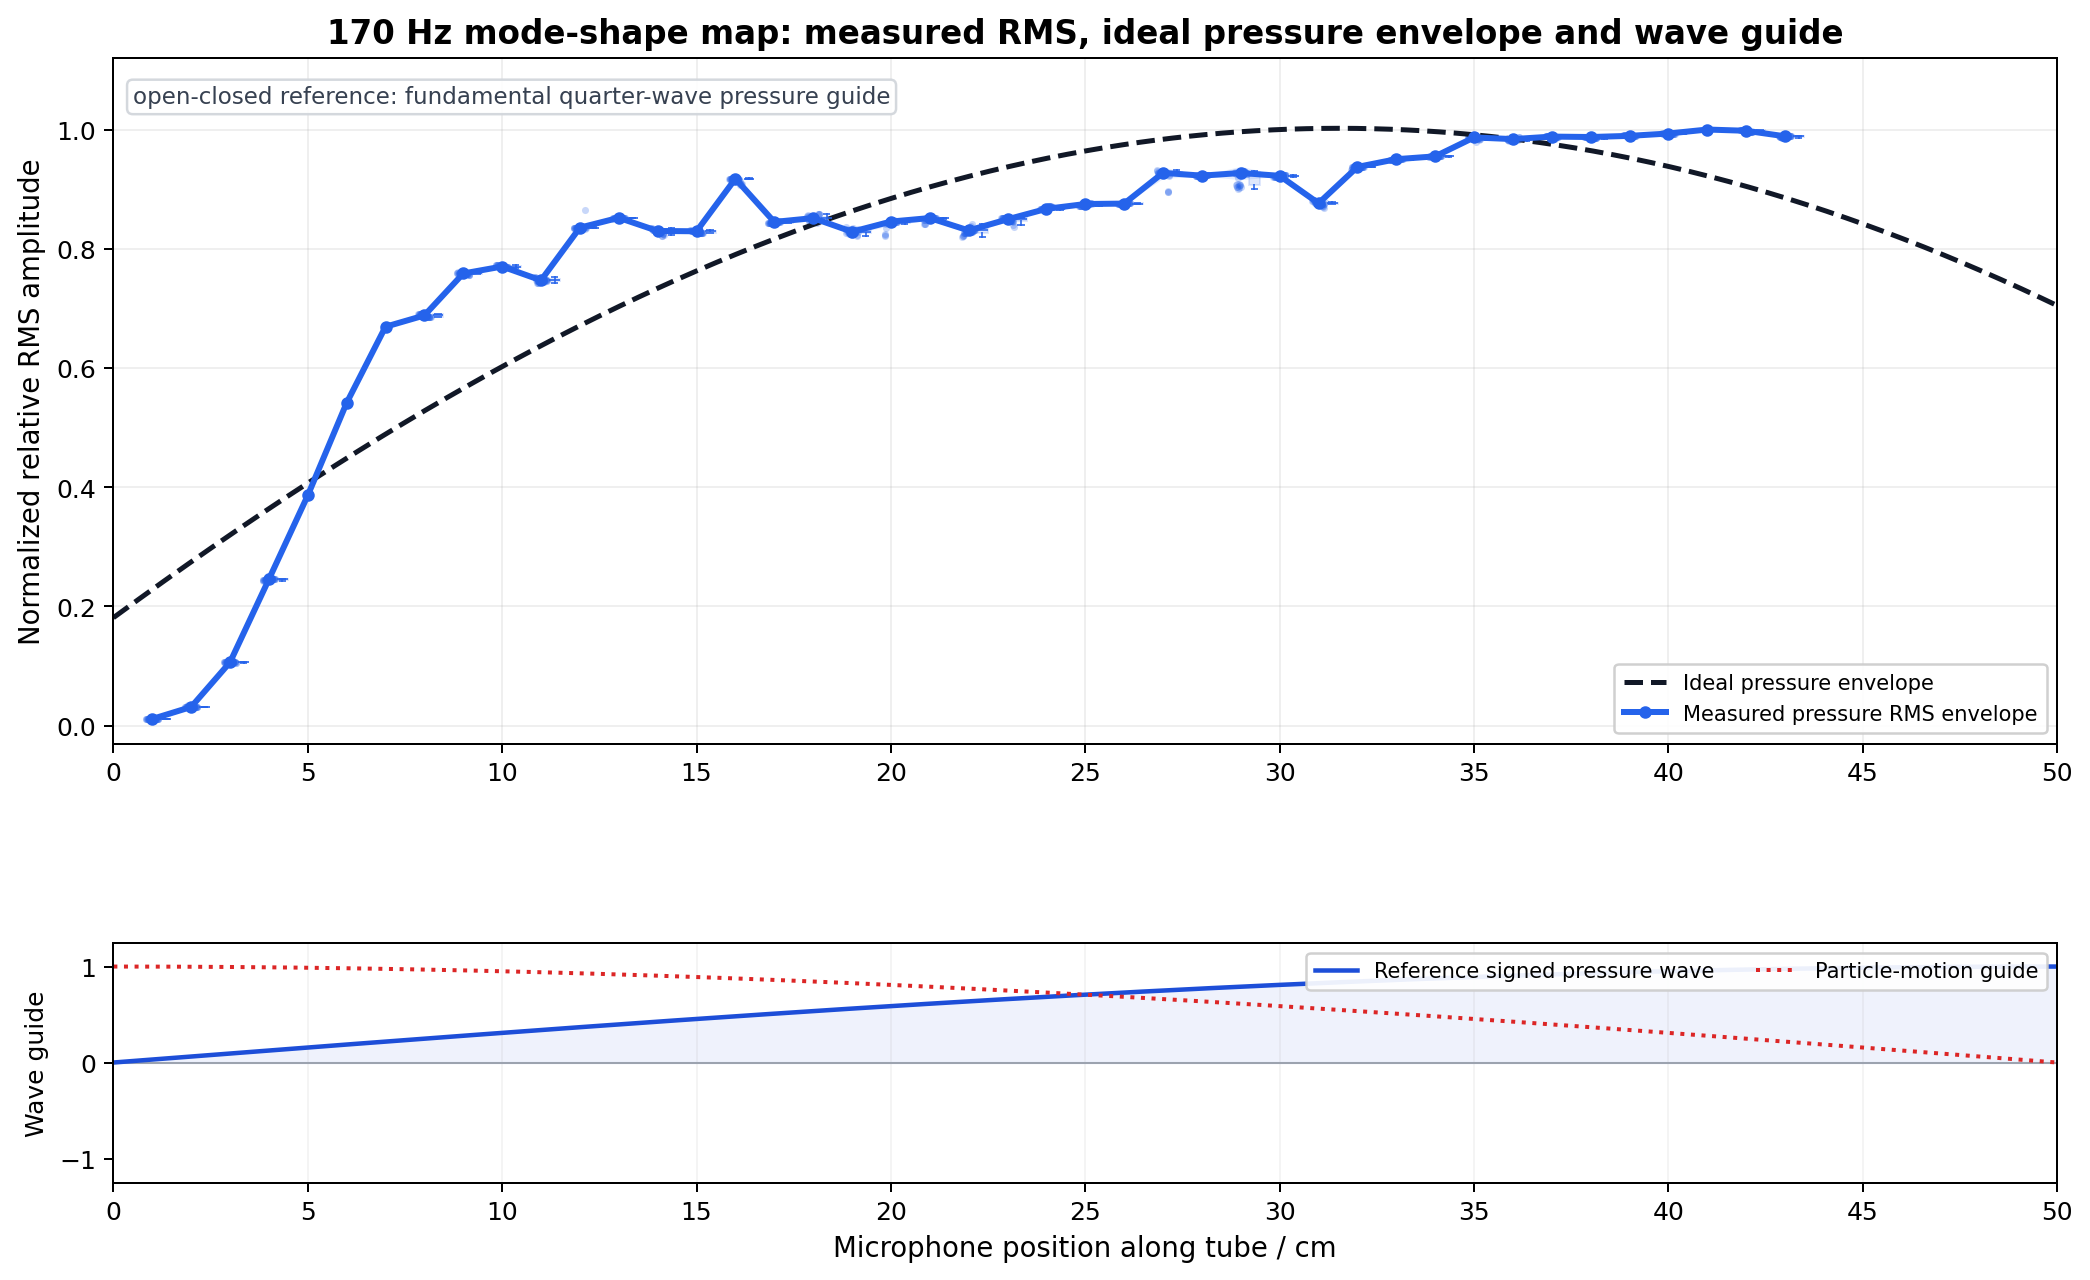
\includegraphics[width=\linewidth]{mode_shape_170Hz_wave.png}
    \caption{\SI{170}{Hz}}
  \end{subfigure}
  \hfill
  \begin{subfigure}{0.49\linewidth}
    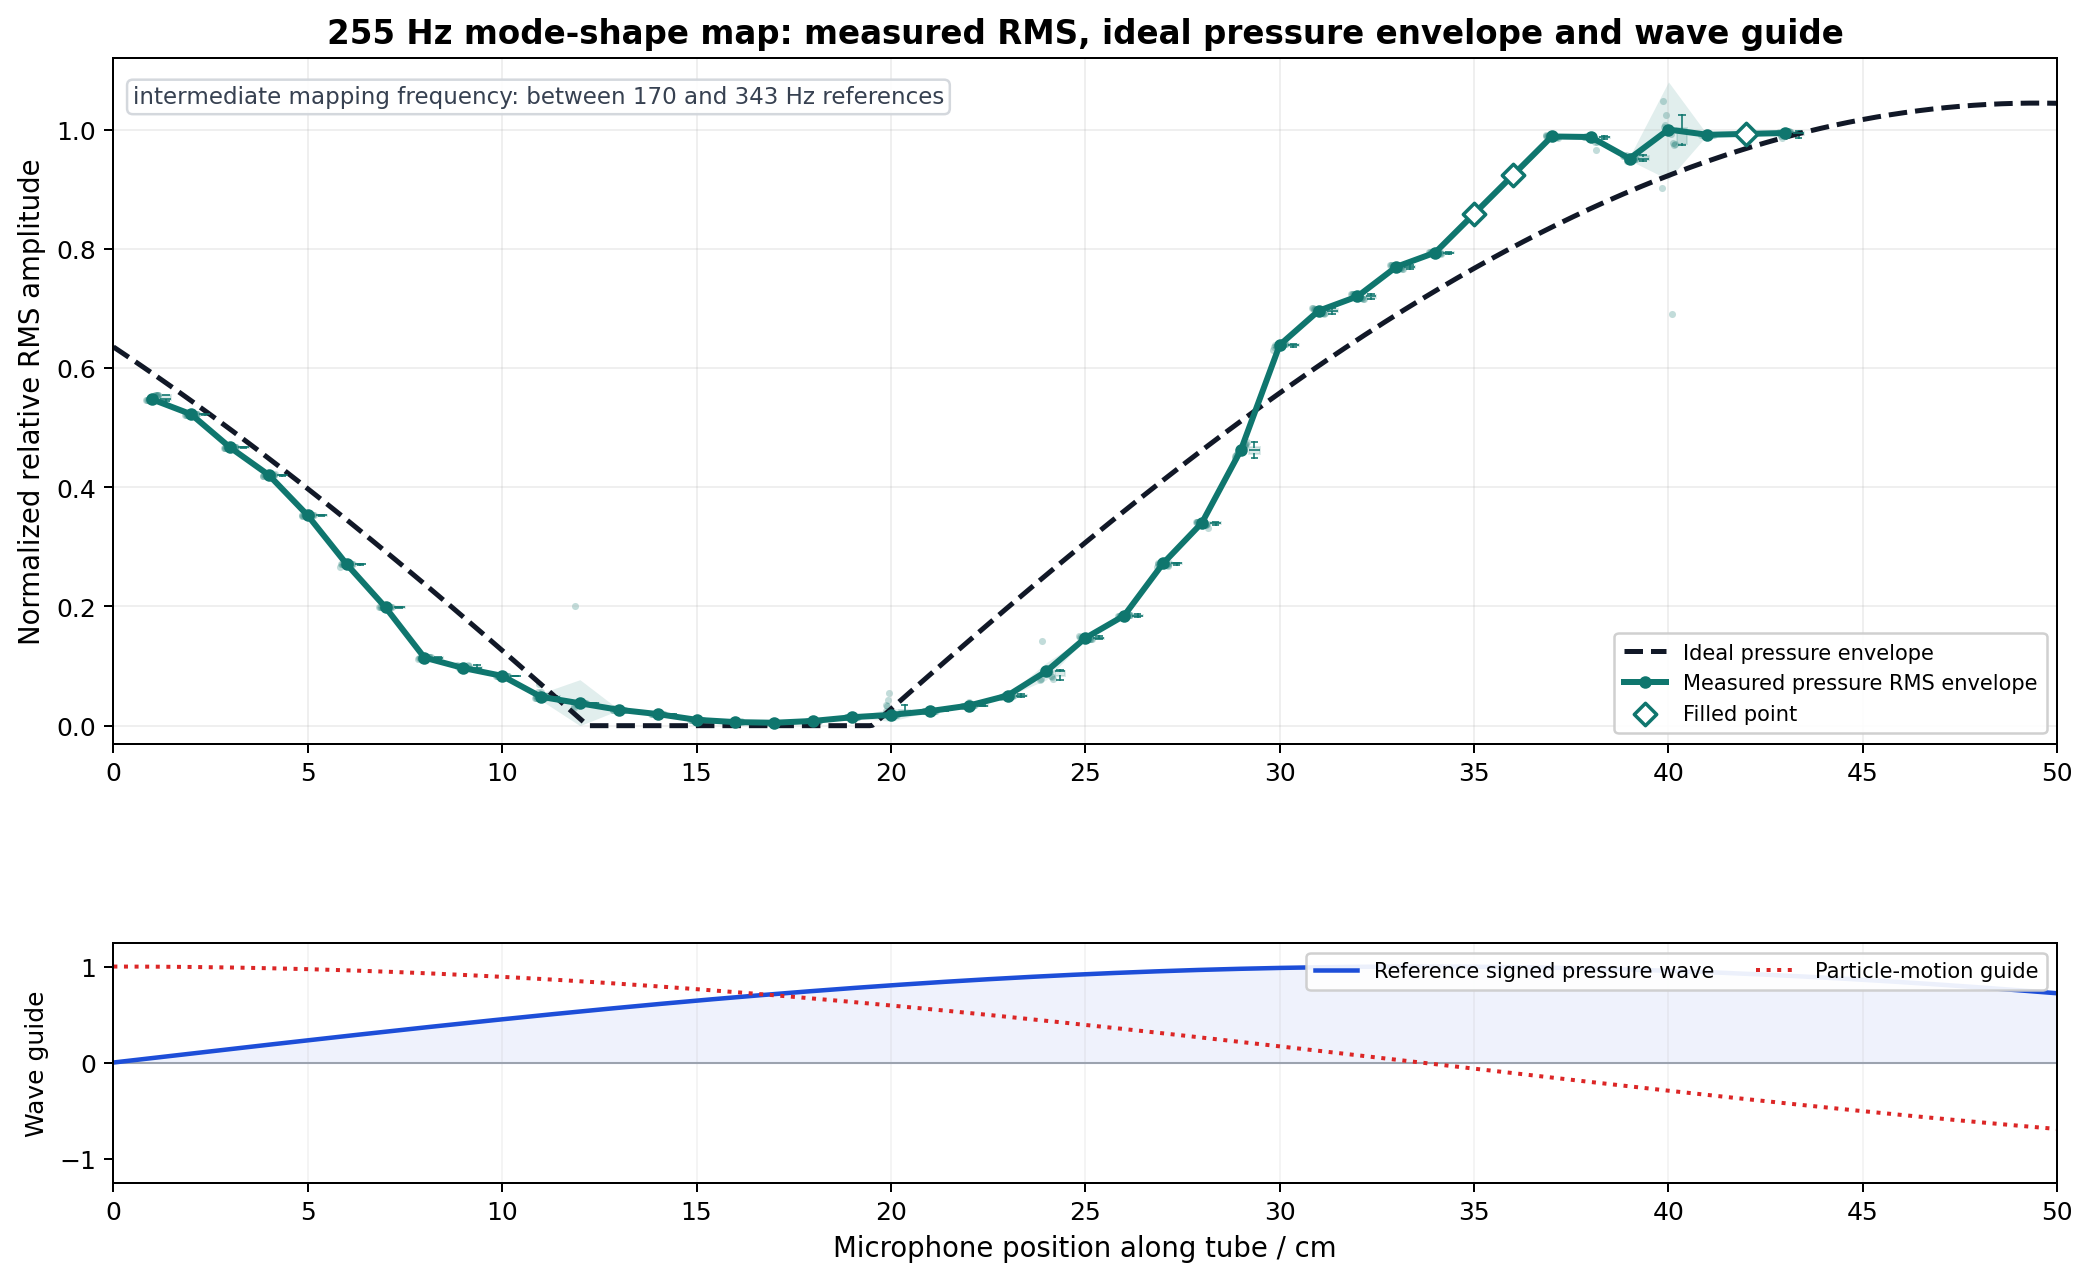
\includegraphics[width=\linewidth]{mode_shape_255Hz_wave.png}
    \caption{\SI{255}{Hz}}
  \end{subfigure}

  \begin{subfigure}{0.49\linewidth}
    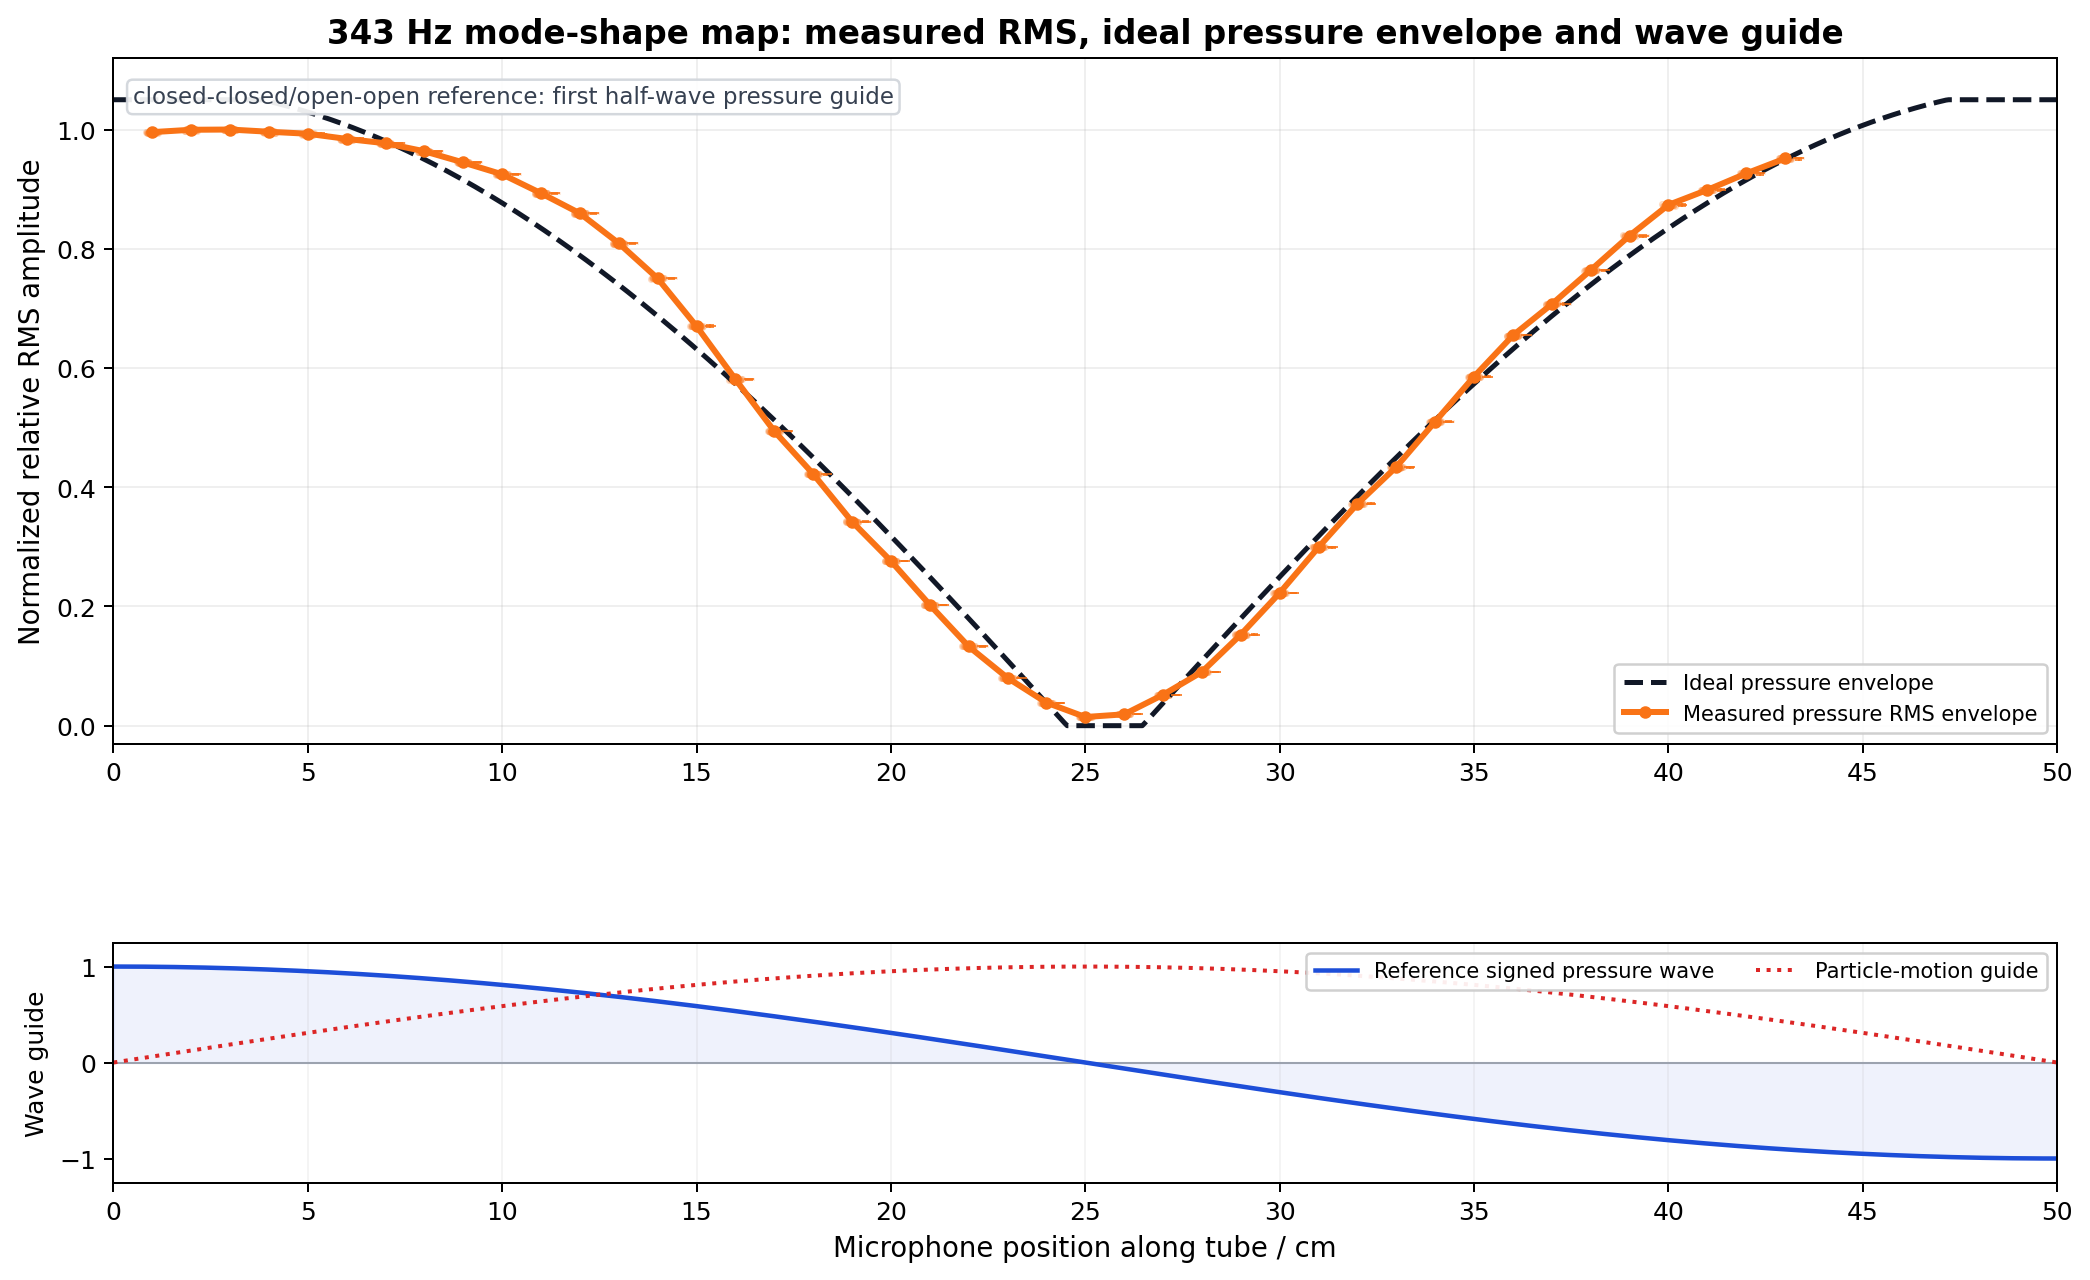
\includegraphics[width=\linewidth]{mode_shape_343Hz_wave.png}
    \caption{\SI{343}{Hz}}
  \end{subfigure}
  \hfill
  \begin{subfigure}{0.49\linewidth}
    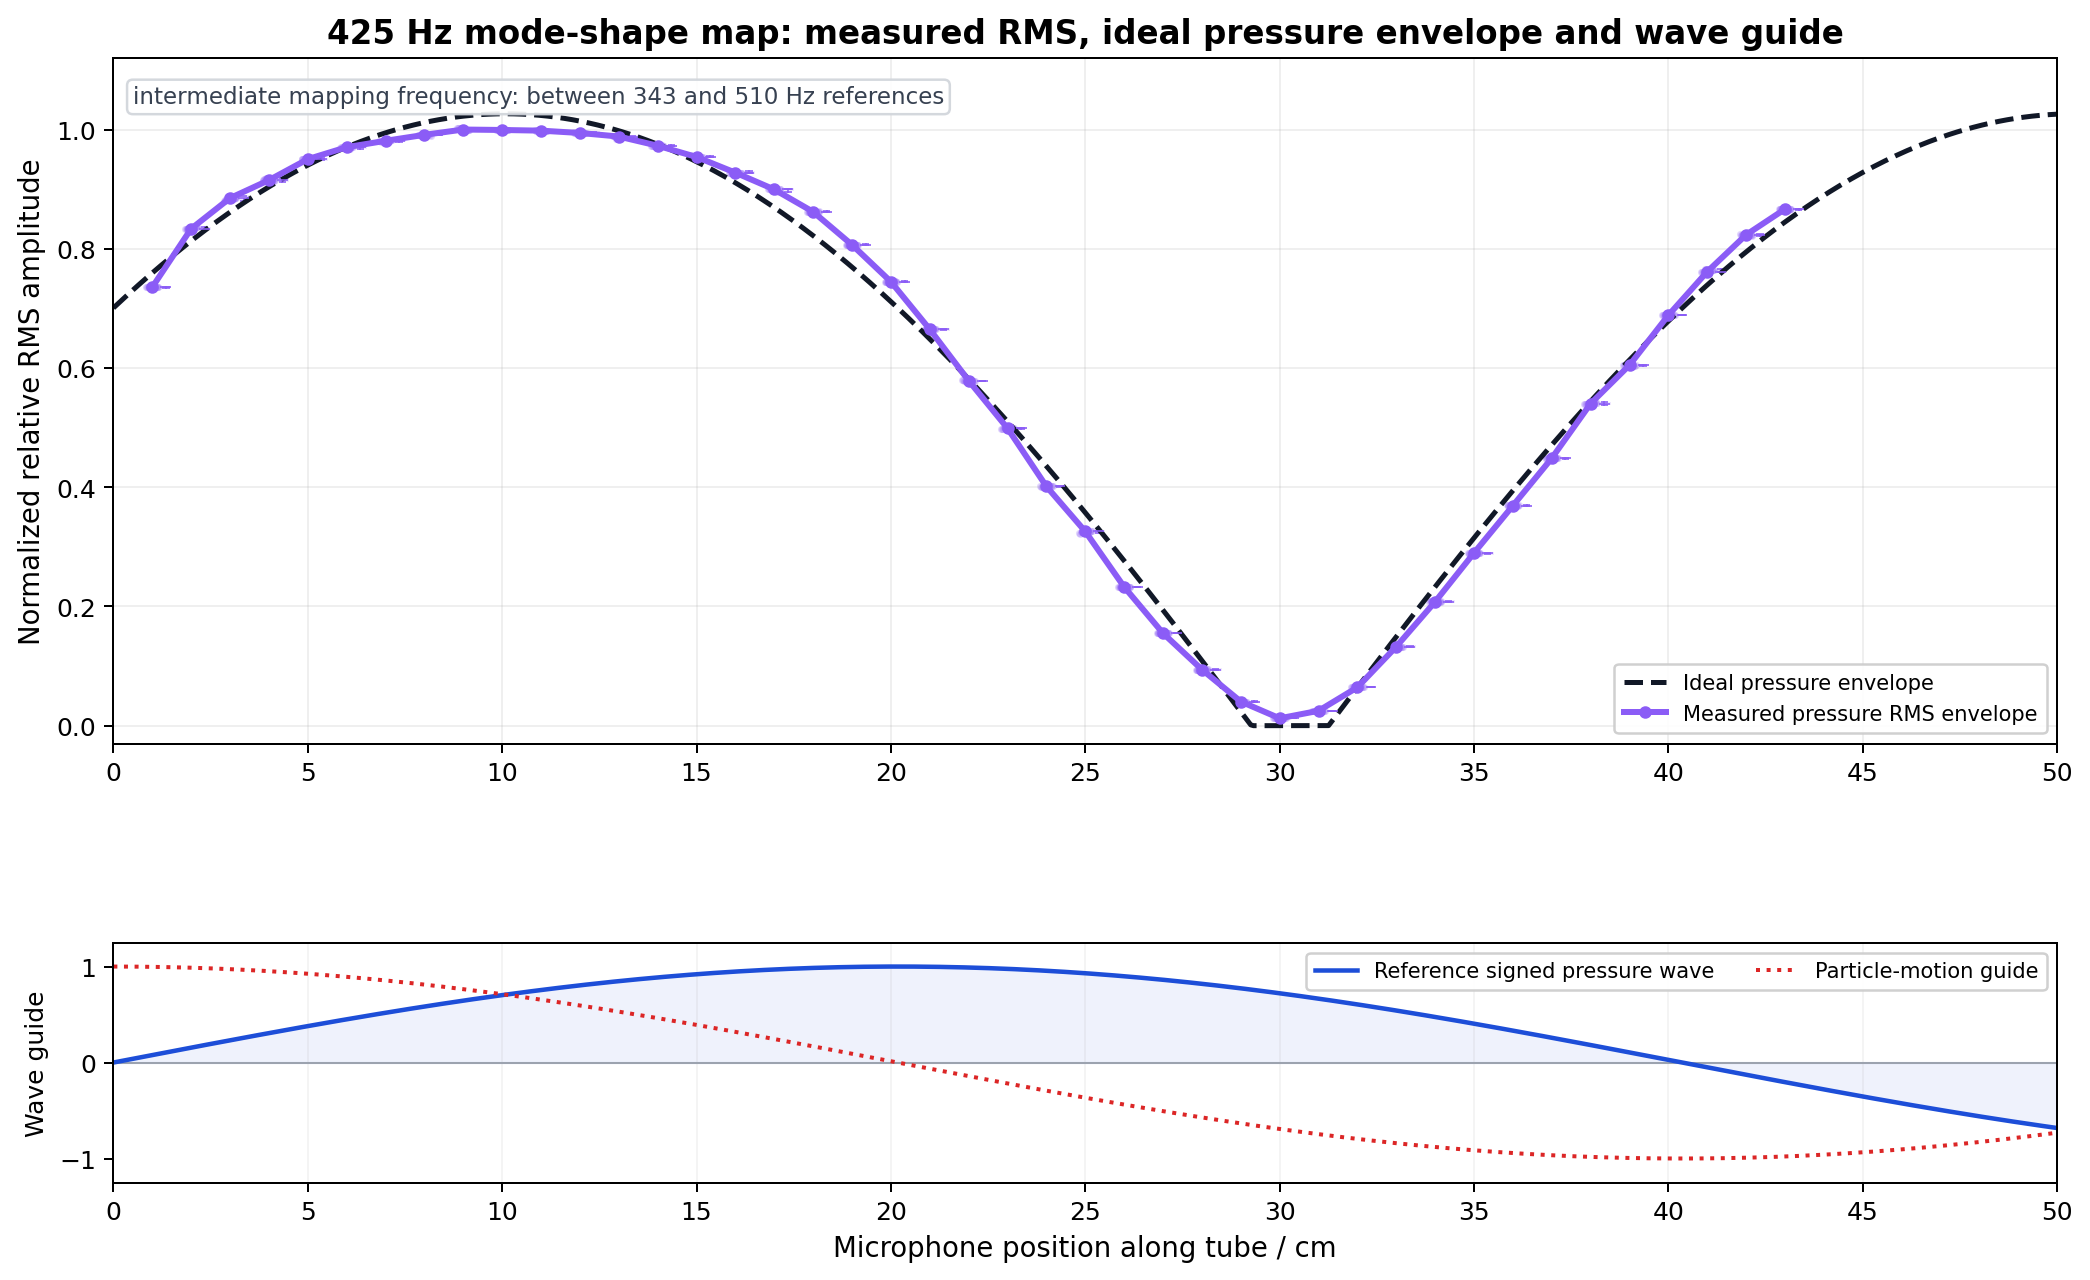
\includegraphics[width=\linewidth]{mode_shape_425Hz_wave.png}
    \caption{\SI{425}{Hz}}
  \end{subfigure}

  \begin{subfigure}{0.49\linewidth}
    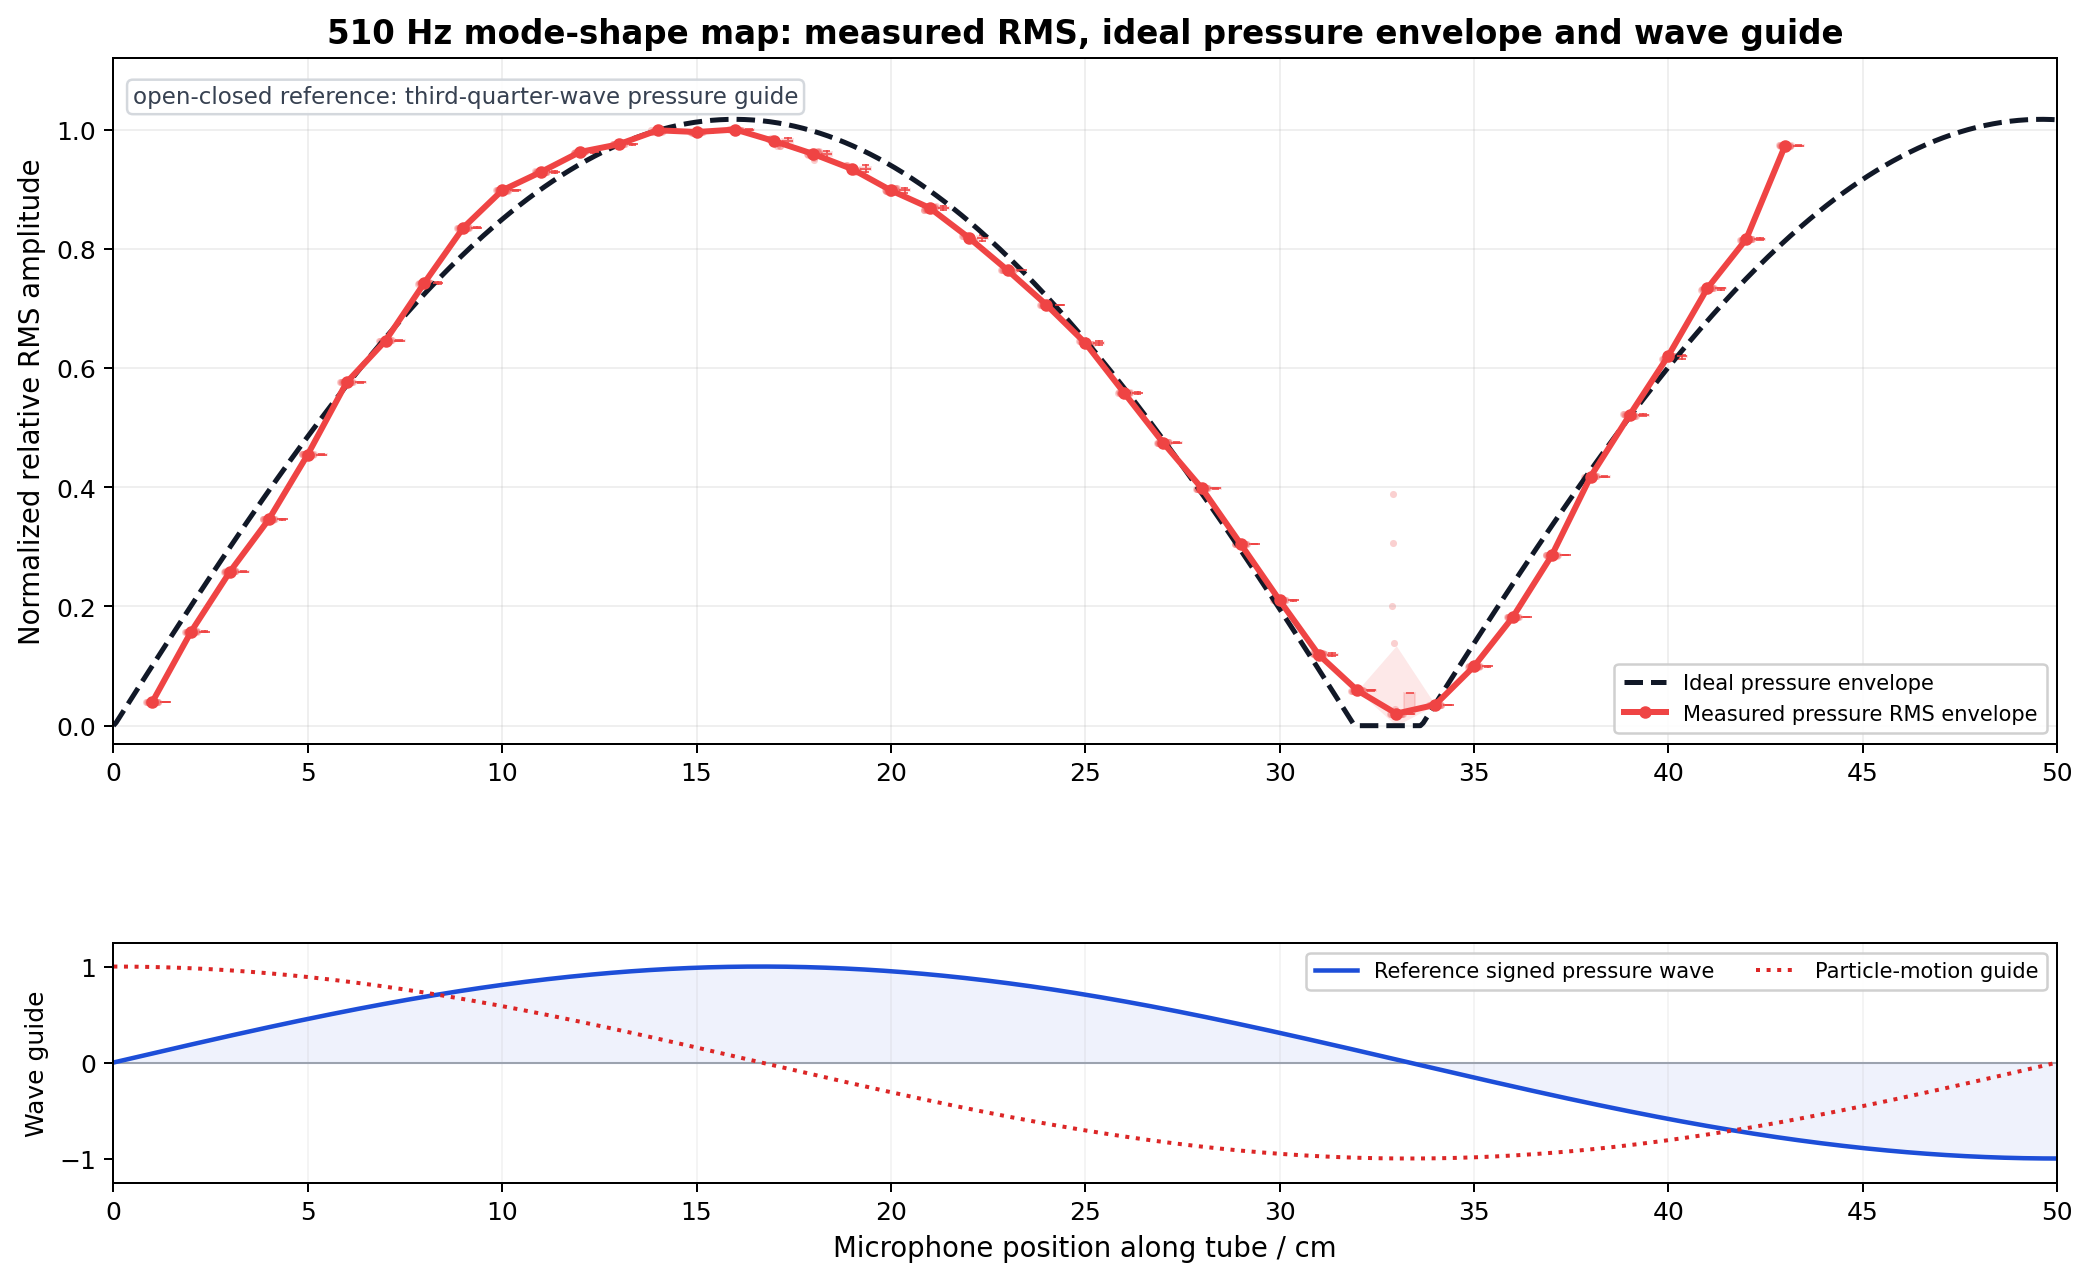
\includegraphics[width=\linewidth]{mode_shape_510Hz_wave.png}
    \caption{\SI{510}{Hz}}
  \end{subfigure}
  \hfill
  \begin{subfigure}{0.49\linewidth}
    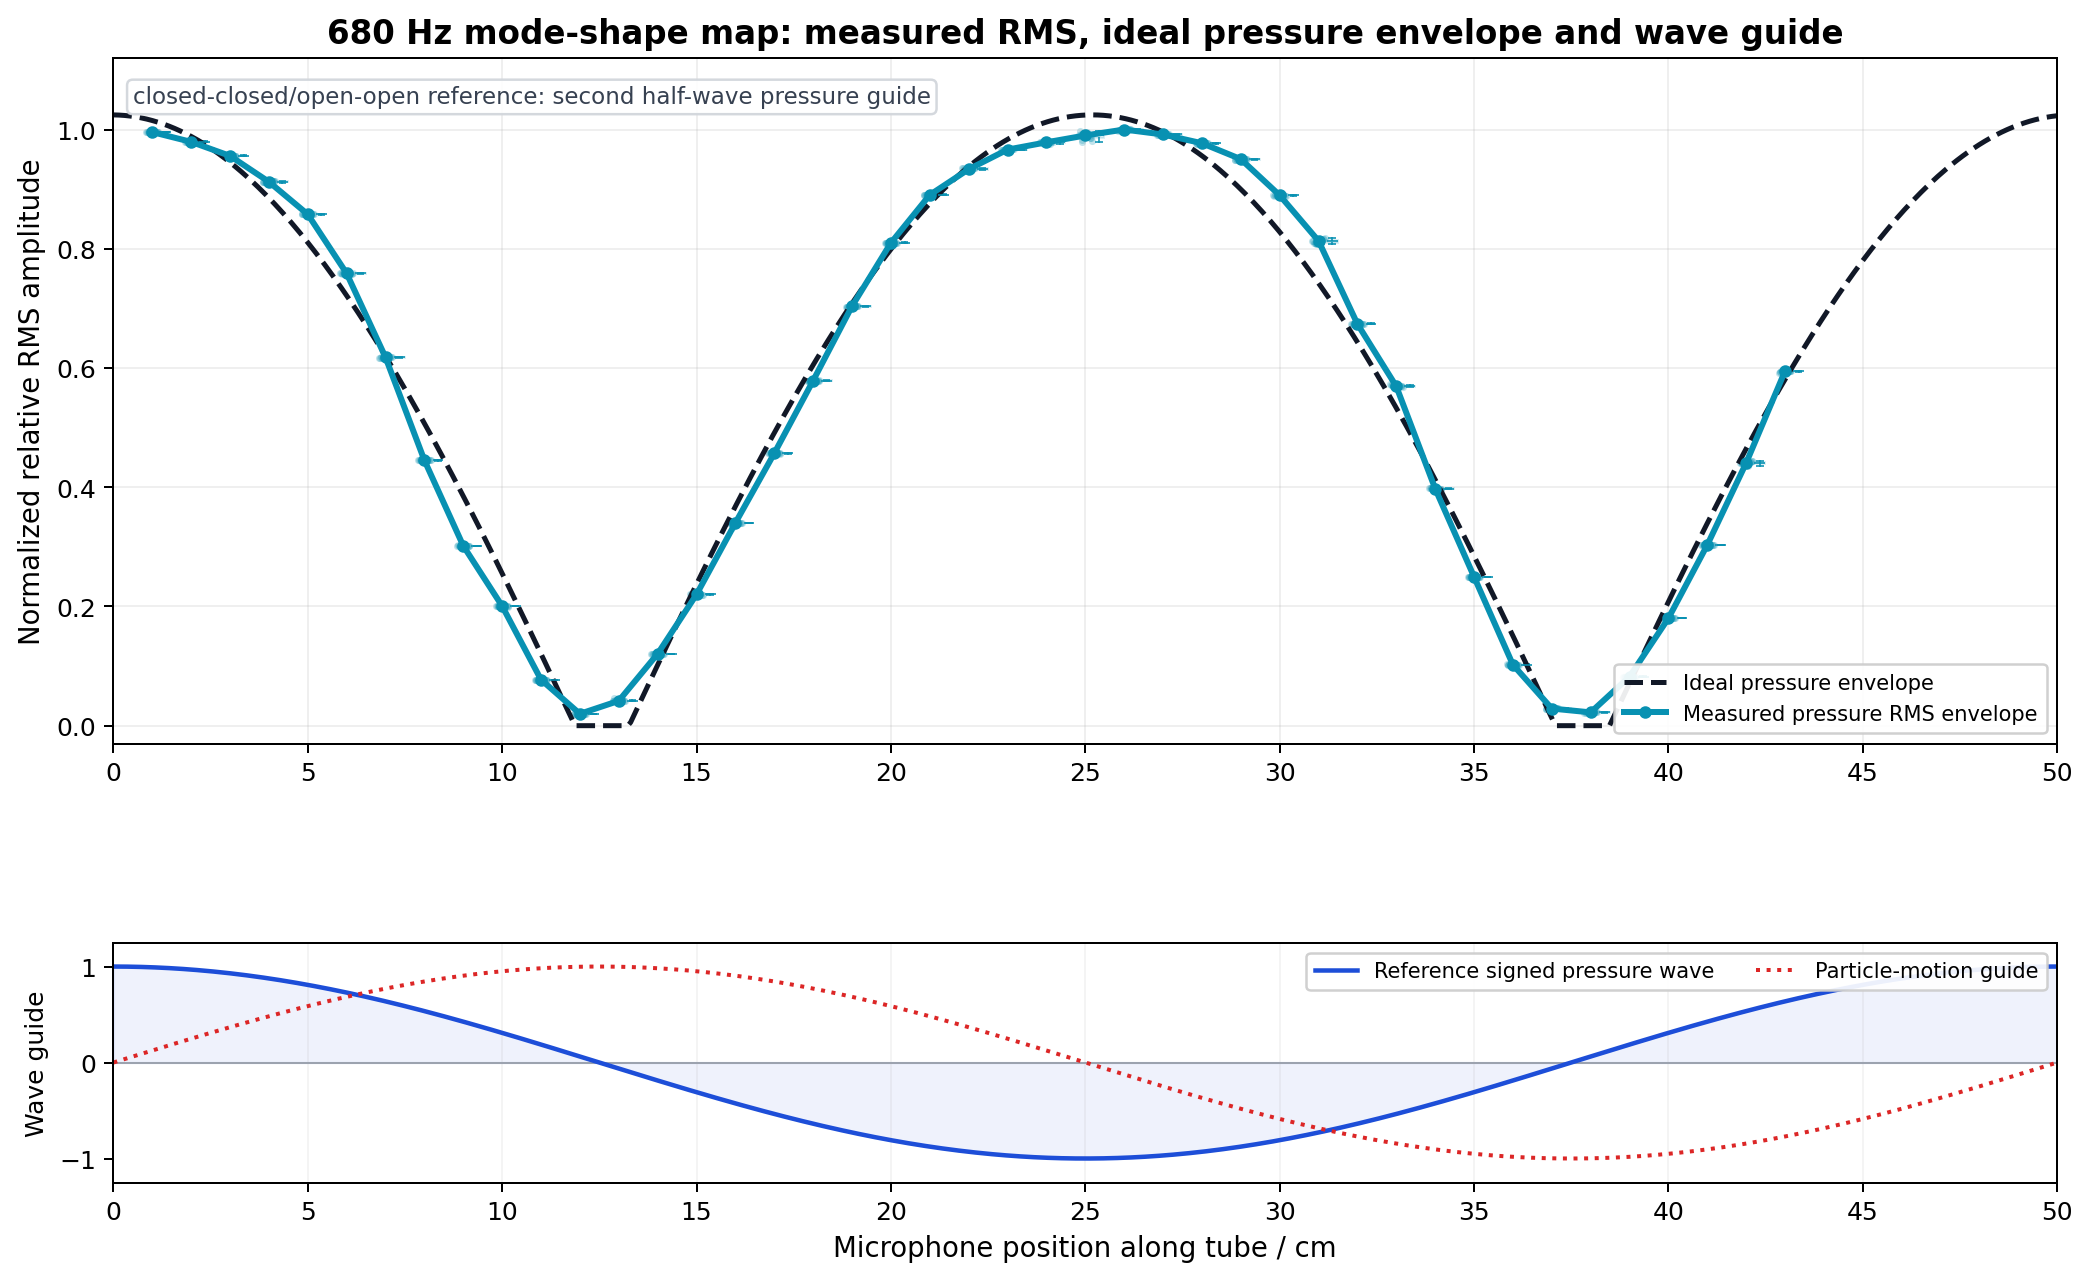
\includegraphics[width=\linewidth]{mode_shape_680Hz_wave.png}
    \caption{\SI{680}{Hz}}
  \end{subfigure}
  \caption{Single-frequency mode-shape plots. The upper panels show measured normalized RMS envelopes. The lower guide strips distinguish signed pressure and particle-motion references.}
\end{figure}

\begin{table}[H]
  \centering
  \caption{Fitted ideal-guide parameters and mean squared error for visual comparison.}
  \begin{tabular}{rrrrr}
    \toprule
    Frequency & MSE & Phase & Offset & Scale \\
    \midrule
    170 & 0.0118 & 5.301 & -0.845 & 1.847 \\
    255 & 0.0071 & 0.830 & -0.214 & 1.258 \\
    343 & 0.0009 & 6.252 & -0.070 & 1.145 \\
    425 & 0.0005 & 5.498 & -0.086 & 1.112 \\
    510 & 0.0016 & 4.791 & -0.089 & 1.106 \\
    680 & 0.0011 & 0.005 & -0.097 & 1.122 \\
    \bottomrule
  \end{tabular}
\end{table}

\section{Discussion}

\subsection{Why the Sweep and Mapping Tell Different Stories}

The sweep result would be misleading if it were read alone. Its largest amplitudes occur in a broad low-frequency band. This band likely contains speaker output, amplifier behavior and sensor response in addition to the tube response. The \SI{343}{Hz} point is low at \(x=\SI{37.5}{cm}\) in the sweep. But the \SI{343}{Hz} position map still shows a clear spatial envelope with a strong low-amplitude region around \SI{25}{cm} and high regions near the scanned ends. This is why mode-shape identification needs spatial mapping rather than one-point loudness.

\subsection{Interpretation of the Six Frequencies}

The \SI{170}{Hz} map is broadly consistent with a low-order quarter-wave-like pressure reference. But it does not behave like a perfect monotonic textbook curve over the whole scanned region. Its fitted-guide MSE is larger than those of the higher-frequency maps. The response also remains high over a wide region after about \SI{12}{cm}. This suggests stronger real-boundary and drive effects. The \SI{255}{Hz} map is best described as an intermediate pattern, not as an exact eigenfrequency. It also contains three interpolated positions and the largest number of clipped raw samples among the final six-frequency set.

The \SI{343}{Hz}, \SI{425}{Hz}, \SI{510}{Hz} and \SI{680}{Hz} maps match the fitted guide curves more closely. Their MSE values are below about 0.002 except for the still-small \SI{510}{Hz} case. Their low- and high-amplitude regions shift in a way that is consistent with increasing spatial order. The \SI{680}{Hz} map shows a strong maximum around \SI{26}{cm} and a low region around \SI{12}{cm} in the scanned coordinate. This indicates a more structured higher-order pattern. These results support standing-wave-like pressure-mode formation, but they still require real-boundary interpretation.

\subsection{Real-Boundary Effects}

The apparatus is not a perfect open-closed or closed-closed tube. The loudspeaker end is not a mathematically open end. It is a driven, coupled boundary. The blocked end includes a board and a probe-access path, so it is not a lossless rigid termination. The microphone itself slightly perturbs the tube. Leakage, bead friction and nonuniform coupling can also shift the measured envelope. For this reason, the report uses both ideal reference families as interpretive guides instead of forcing all frequencies into one exact boundary model.

\section{Limitations and Uncertainty}

\begin{itemize}
  \item The KY-037 output is a relative voltage indicator, not calibrated SPL and not absolute pressure.
  \item Different drive volumes were used for practical measurement, so cross-frequency amplitude comparison must use normalized shapes rather than raw amplitude.
  \item The accessible scan range in the cleaned analysis was \SIrange{1}{43}{cm}, not the full \SI{50}{cm} physical tube length.
  \item The \SI{255}{Hz} row includes three linearly interpolated positions: \SI{35}{cm}, \SI{36}{cm} and \SI{42}{cm}.
  \item Beads provide qualitative visual evidence only; they are affected by particle motion, accumulation, friction, static charge and lighting.
  \item The fixed-position sweep was limited to its sampled frequency set; \SI{425}{Hz} and \SI{680}{Hz} are not directly represented as exact rows in the sweep summary used here.
  \item More repeated full position scans would allow stronger uncertainty estimates and repeatability analysis.
\end{itemize}

\section{Conclusion}

The experiment supports the formation of standing-wave-like acoustic pressure patterns in a real loudspeaker-driven acrylic tube. The ideal formulas for open-closed and closed-closed/open-open tubes provided useful candidate frequencies for a \SI{50}{cm} tube. But the real apparatus showed mixed-boundary behavior rather than one exact textbook model. Bead visualization gave qualitative evidence that the spatial pattern changes with drive frequency. The fixed-position sweep showed that one-point amplitude is strongly affected by system response and local position, so it cannot identify mode shape by itself. The frequency-position RMS maps provided the main quantitative evidence. The normalized pressure-amplitude envelopes at \SI{170}{Hz}, \SI{255}{Hz}, \SI{343}{Hz}, \SI{425}{Hz}, \SI{510}{Hz} and \SI{680}{Hz} showed frequency-dependent high and low regions consistent with standing-wave-like mode formation. The strongest final interpretation is therefore not that the tube exactly reproduces ideal modes, but that ideal mode families are useful references for understanding measured pressure envelopes in a non-ideal, loudspeaker-driven resonator.

\appendix
\section{Data and Processing Sources}

The data files, figure files, and calculation scripts used for this report are available in the GitHub repository:
\url{https://github.com/gary1110086/standing-wave-mode-mapping-data}.

The exact repository version used for this report is commit \texttt{83644df9b9cdf20baae3d6afbe5d49d3562cde01}.

\begin{itemize}
  \item Primary mode-shape data: \path{data/mode_shape/mode_shape_6freq_normalized_summary.csv}.
  \item Row-normalized heatmap table: \path{data/mode_shape/mode_shape_6freq_row_normalized_heatmap_table.csv}.
  \item Fit parameter source: \path{data/mode_shape/ideal_reference_fit_parameters.csv}.
  \item Fixed-position sweep source: \path{data/frequency_sweep/frequency_response_summary.csv}.
  \item Report figures: \path{figures/} and \path{report/figures/}.
  \item Sensor description in this report uses KY-037 or microphone sound detection sensor.
\end{itemize}

\end{document}
